\chapter{OVERVIEW OF PHOTOGRAPHIC CENSUSING} \label{chapter:overview}

\noindent Animal population monitoring is hard to do at large scales because it is immensely laborious for ecologists.  It is often too overwhelming and tedious to track hundreds -- let alone thousands -- of animals with invasive tools like ear tagging and GPS collars.  Furthermore, historical methods like aerial surveys and hand-based counts lack the ability to recognize individual animals over time, severely limiting the potential to establish ecological trends.  Knowing an animal population through the majority of its members, in contrast, provides crucial insight.  For example, ecologists gain a more intimate and timely understanding of a species' health when they can determine life expectancy, visualize migration patterns, and quickly measure the effectiveness of conservation policy.  A comprehensive database of animal IDs is, therefore, a powerful tool for monitoring an endangered population, and the question is, ``\textit{what is the best way to build one?}''  Unfortunately, a large database of IDs cannot be built by hand because the amount of work required to curate it is too prohibitive as the database grows.  What is needed for sustainable population monitoring is automation.  Any end-to-end solution to the problem of large-scale population monitoring must fundamentally be built around maximizing the completeness of an ID database while minimizing the amount of human effort needed to create it.

This chapter introduces the concept of \textit{photographic censusing}\footnote{As a process that is powered by computer vision algorithms, animal population censusing was first explored in the author's master's thesis~\cite{parham_photographic_2015}.  It is formally proposed and described here as a self-contained and complete methodology.}, a comprehensive and automated procedure for large-scale animal population monitoring.  The methodology uses digital images of animals as input, machine learning algorithms to automate their analysis, an ID database to track sightings of individual animals, and a management algorithm to control when human interaction is needed.  Furthermore, photographic censusing is intended to be feasible for resource-strapped organizations to implement for large species and migratory ranges.  As we will see, photographic censusing has been experimentally validated \textit{in situ} on a wild animal population with thousands of individual members across 25,000 square kilometers.  Photographic censusing is also intended to be used with open populations, with some animals only seen once (what we will call ``singletons'') and others seen many times (``multitons'').  This chapter begins with an overview of photographic censusing and discusses real-world challenges and considerations when high degrees of automation are needed.  Next, an enumerated list of the required machine learning and management algorithms is provided, and a mathematical framework is introduced for estimating the size of an animal population when automated components are involved.  Lastly, a new evaluation database is proposed containing hundreds of animal IDs with multiple sightings, some over two years, for the endangered Gr\'evy's zebra species in Kenya.

\section{Problem Description}

Photographic censusing produces a population estimate by performing a sight-resight study (see Section~\ref{sec:capture-mark-recapture}).  A sight-resight study is based on the sampling statistics of capture-mark-recapture and, as a result, is constructed from an initial collection of photographs followed by a second, independent, and comparable collection.  The image data needed for photographic censusing is gathered through a \textit{photographic censusing rally}, an event where volunteer ``citizen scientist'' photographers are trained to take pictures of the desired species and tasked to cover its residential area for two back-to-back days.  The question is, given a large collection of images taken during a two-day censusing rally, ``\textit{how many individuals are in the population?}''  Photographic censusing answers this question by building a comprehensive database of animal IDs with the help of automated tools.  The ID database is curated by comparing different pairs of sightings to determine which show the same animal or not. The process concludes when a management algorithm is satisfied with the level of redundancy and consistency for all IDs in the database.  By comparing the ratio of animal IDs seen on day 1, seen on day 2, and seen on both days, the total number of animals in the population is estimated.  This process can rely heavily on human decision-making, so the overall significance of photographic censusing as a solution is fundamentally tied to how automatically it can produce a reliable database of animal IDs.

Since automation is crucial, we need to discuss what kinds of machine learning algorithms are needed and consider how they may fail, resulting in a need for human involvement.  The methodology of photographic censusing is built on analyzing digital images, and, therefore, it is appropriate that computer vision algorithms should be considered primarily for its automation needs.  For example, the detection pipeline (discussed in Chapter~\ref{chapter:detection}) is used to automatically filter the collected images into a set of relevant animal sightings.  As we will see, however, additional computer vision algorithms are also needed to identify potential matches and verify pairs of annotations.  Furthermore, computer vision algorithms are imperfect, and curating an ID database requires human effort to fill the accuracy gap.  As such, there are three specific and systemic challenges encountered during automated ID curation that we must discuss because they drastically increase the need for human interaction: 1) the proper selection of annotations from the detection pipeline, 2) the correct matching of the intended animals within annotations, and 3) the managing of ID curation and deciding when a human needs to do additional ID verification.  Unfortunately, the amount of human effort required can be substantial when poor-performing computer vision algorithms are used and these sources of error are not appropriately addressed.  The following sub-sections describe these problems and explain why they dramatically hinder the automation -- and therefore the general usefulness -- of photographic censusing.

\begin{figure}[!t]
    \begin{center}
        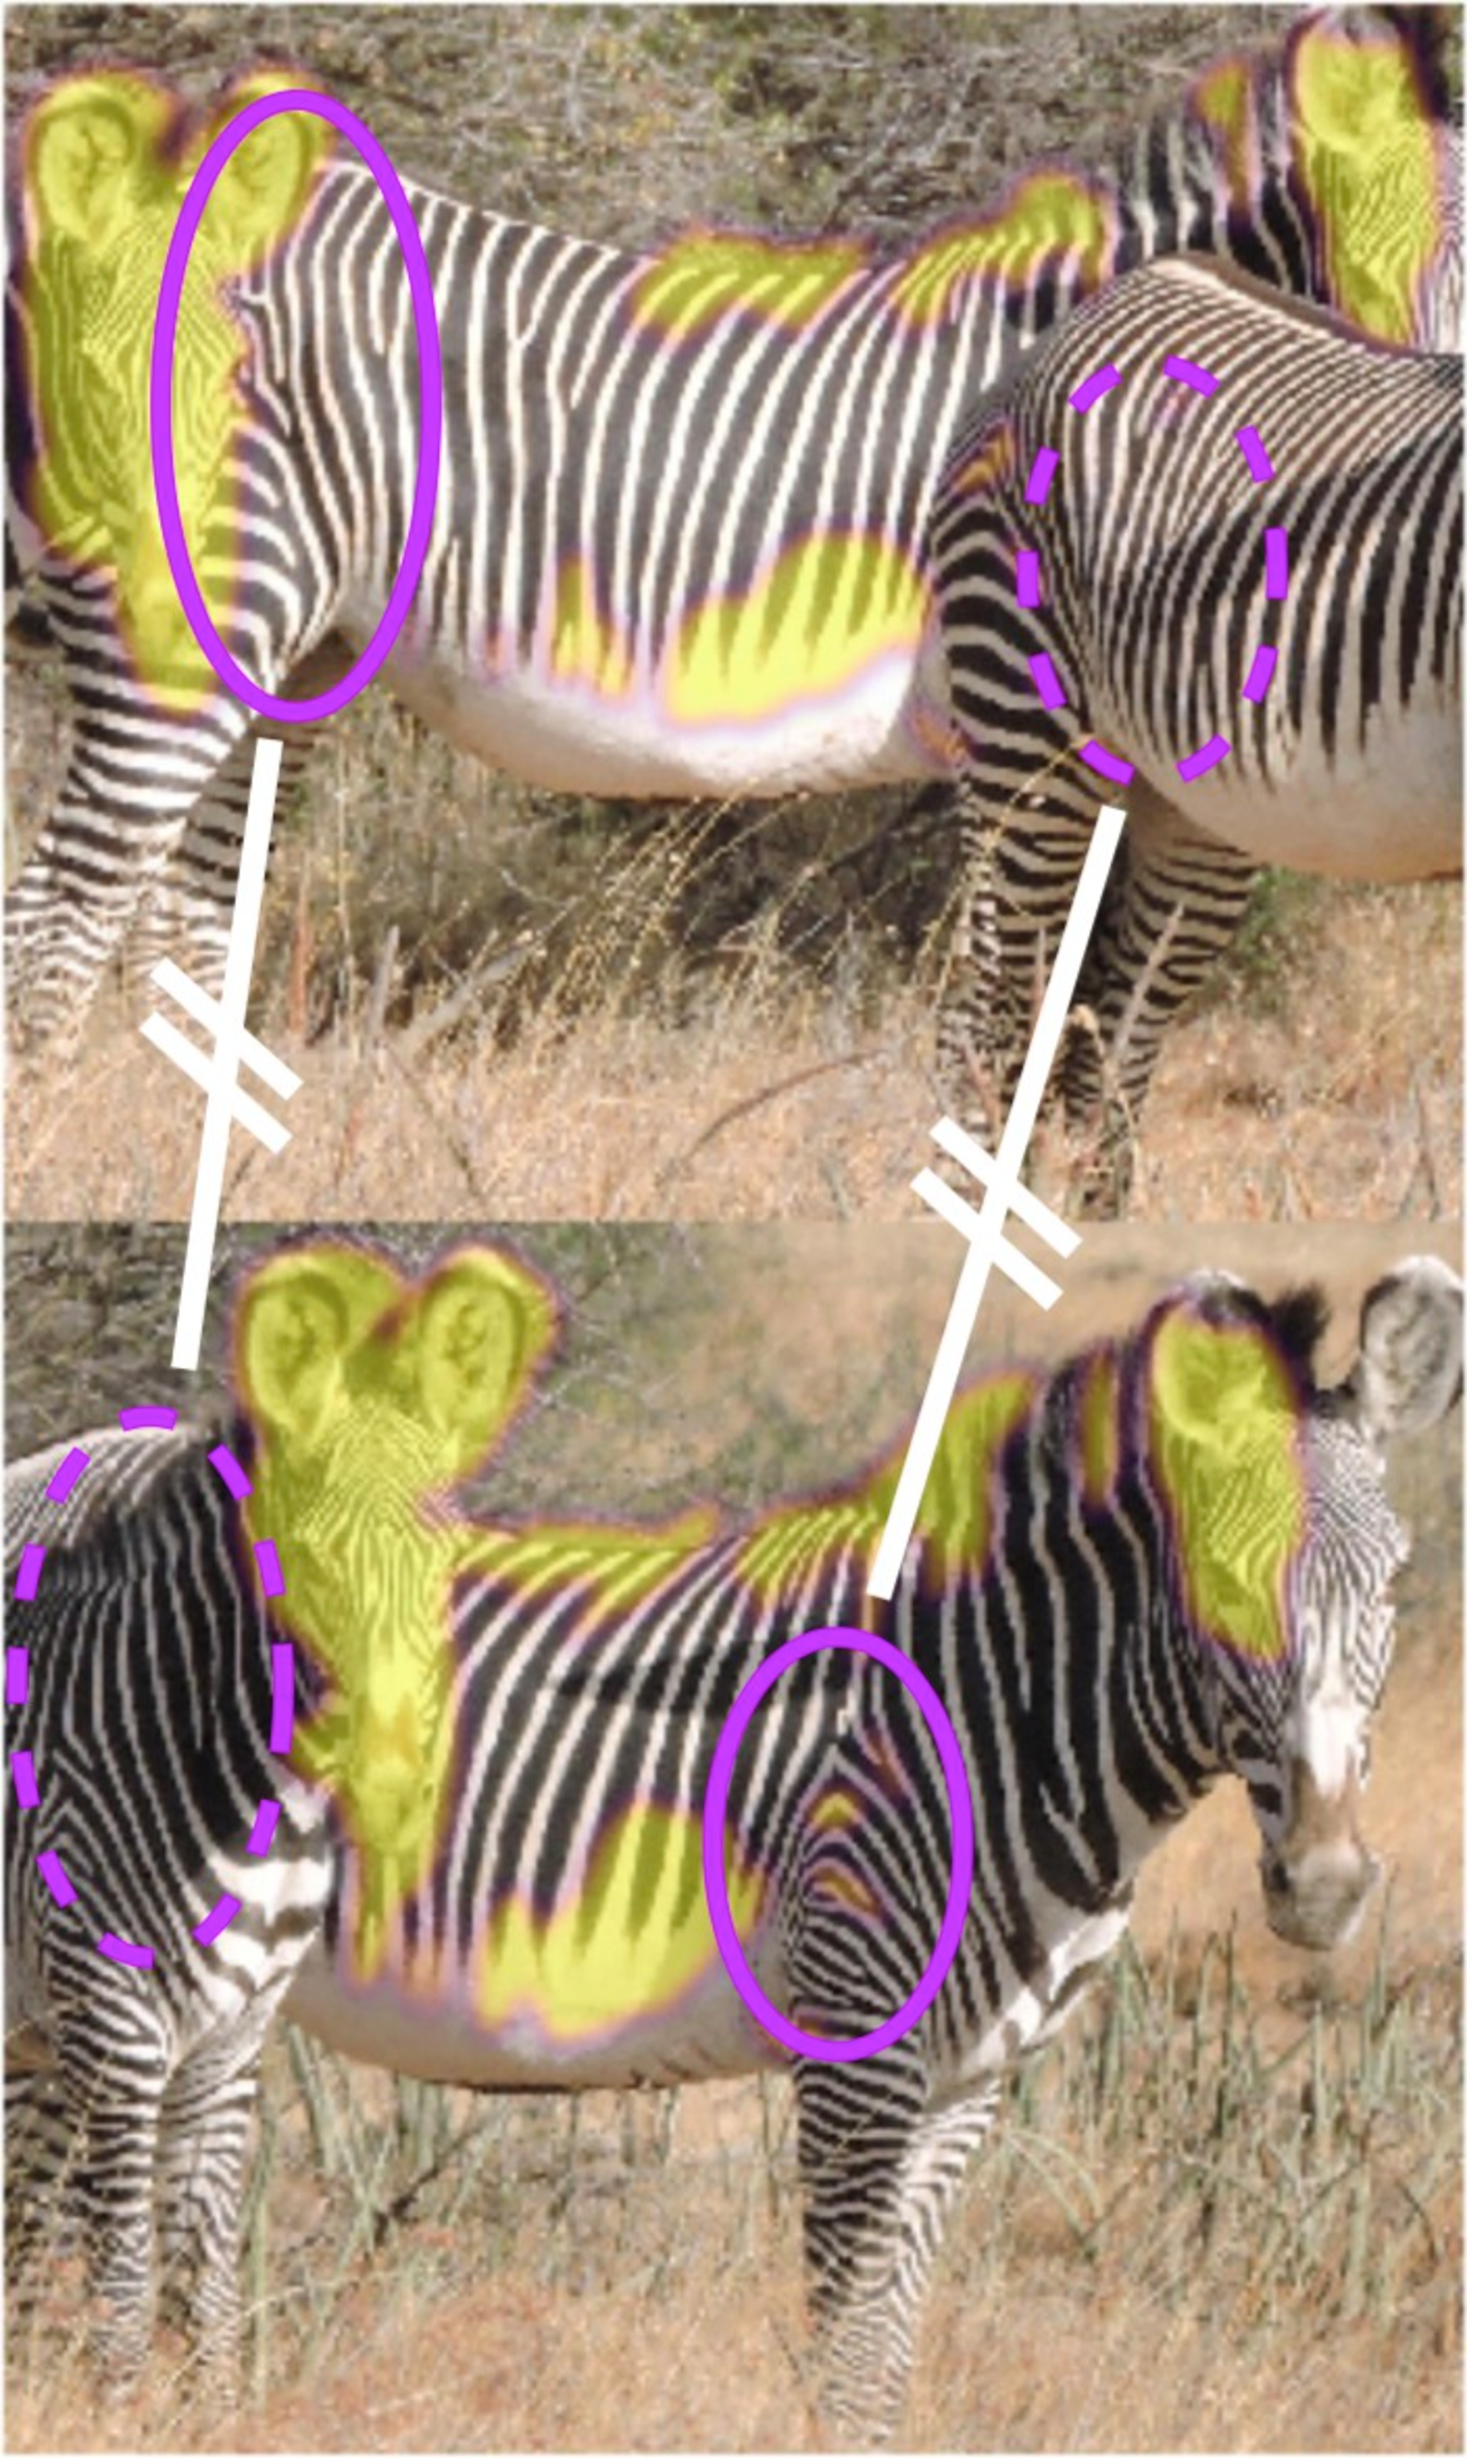
\includegraphics[width=0.67\linewidth]{resources/ca-cannottell.pdf}
    \end{center}
    \caption{An example images of an incomparable match, where the background animals are being compared but a decision cannot be reliably made.  The distinctive visual regions that are normally used for verification (the purple oval regions) are both occluded.}
    \label{fig:ca-cannottell}
\end{figure}

\subsection{Which Annotations to Select: Comparable Annotations}

The first problem we must consider is the selection of which annotations to use for photographic censusing.  To do this, we need to understand how annotations are actually used: annotations are automatically ranked to find potential matches, and algorithms and humans verify the resulting pairs of annotations.  With this in mind, what can we conclude when a given pair of two annotations fail to match?  Does the pair indeed show two different animals?  Not necessarily; there are three distinct possibilities for why two annotations may not match, either 1) the detection pipeline failed to filter at least one of the annotations properly (e.g., poor quality or incompatible viewpoints), 2) the annotations were appropriately filtered and actually showed different animals, or 3) the annotations were filtered correctly but are not \textit{comparable}.  Therefore, we can only conclude that two annotations truly show different animals if they are both comparable, showing the same areas of distinguishing information that can be compared and contrasted.  Since matching is akin to ``marking'' an animal in a sight-resight study, it is essential to approach and define comparability as a distinct property of an individual annotation.  If both annotations in a pair are comparable, a confident and repeatable decision should be possible given enough time to review the pair, regardless of the skill of a particular reviewer.  Furthermore, by not considering comparability, we are potentially allowing ambiguity to enter the ID database.

We would prefer to construct an automated photographic census with annotations guaranteed to be comparable for all potential pairings.  By definition, an annotation is comparable if it provides enough visual information to a reviewer such that a ``same animal'' or ``different animals'' decision is \textit{always} possible.  To provide a counter-example, an \textit{incomparable} match can be seen in Figure~\ref{fig:ca-cannottell}, where the two annotations are exceedingly difficult to compare and would likely be set aside for human review.  The distinction of needing ``enough'' visual information to feel comfortable can be challenging to implement in practice.  Finding the right combination of required visual features is subjective and is unfortunately unique for each species.  For example, the identifying information for a Gr\'evy's zebra is often concentrated in the back hip region and the shoulder chevron at the top of the front leg (e.g., the purple oval regions in Figure~\ref{fig:ca-cannottell}).  Humans commonly use these two areas to verify if a pair of Gr\'evy's zebra annotations are the same or not, and not being able to compare or contrast these regions makes the match much more difficult (or impossible) to decide.  This dynamic suggests a trade-off exists between 1) a complete review of all the detected annotations and 2) the desire to increase the automation of the photographic census.

Unfortunately, not all annotations created by the detection pipeline (and properly filtered for relevant species and viewpoints) are guaranteed to be comparable.  The need for comparability will be addressed in Chapter~\ref{chapter:ca} where the notion of a Census Annotation (CA)\footnote{The motivation of CA is slightly different from Annotation of Interest because comparability does not make an image-level determination and focuses entirely on the annotation.  For example, while an AoI may show enough information to identify it \textit{most} of the time, that does not guarantee that it will be universally comparable \textit{all} of the time.} is introduced and added as a new animal detection component.  The discussion there will demonstrate that photographic censusing is significantly more automated and maintains the same level of accuracy in its population estimate when only Census Annotations are used.

\subsection{Systematic Ranking Errors: Incidental Matching}

Even with a detection pipeline that can accurately find, label, and identify relevant sightings (and filtering methods like Census Annotation to discern the comparable annotations), it is still possible to have considerable problems during automated ID curation.  The second systemic error we must consider happens when a ranking algorithm (see Section~\ref{sec:id_verification}) confidently matches two annotations that do not show the same animal.  This problem results in errors in the ID database because two distinct animal IDs are then incorrectly and automatically merged.  This problem is called ``incidental matching'.  In order to rely on high amounts of automation during photographic censusing, we need to examine the two most common incidental matching scenarios, photobombs~\cite{crall_identifying_2017} and scenery matches, and review why they happen.

\begin{figure}[!t]
    \begin{center}
        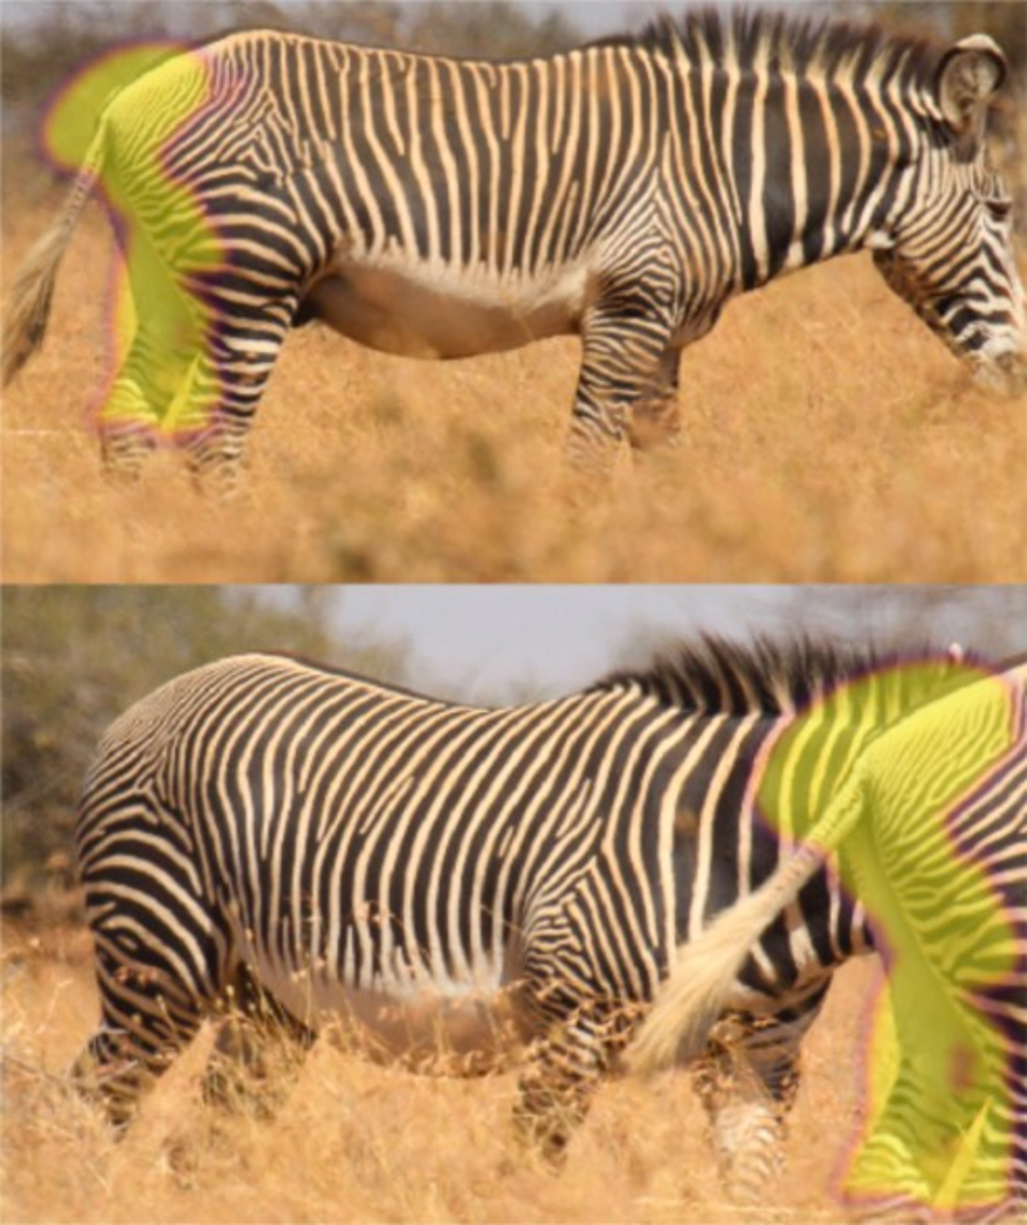
\includegraphics[width=0.4\linewidth]{resources/photobomb.pdf}
        \hspace{0.5cm}
        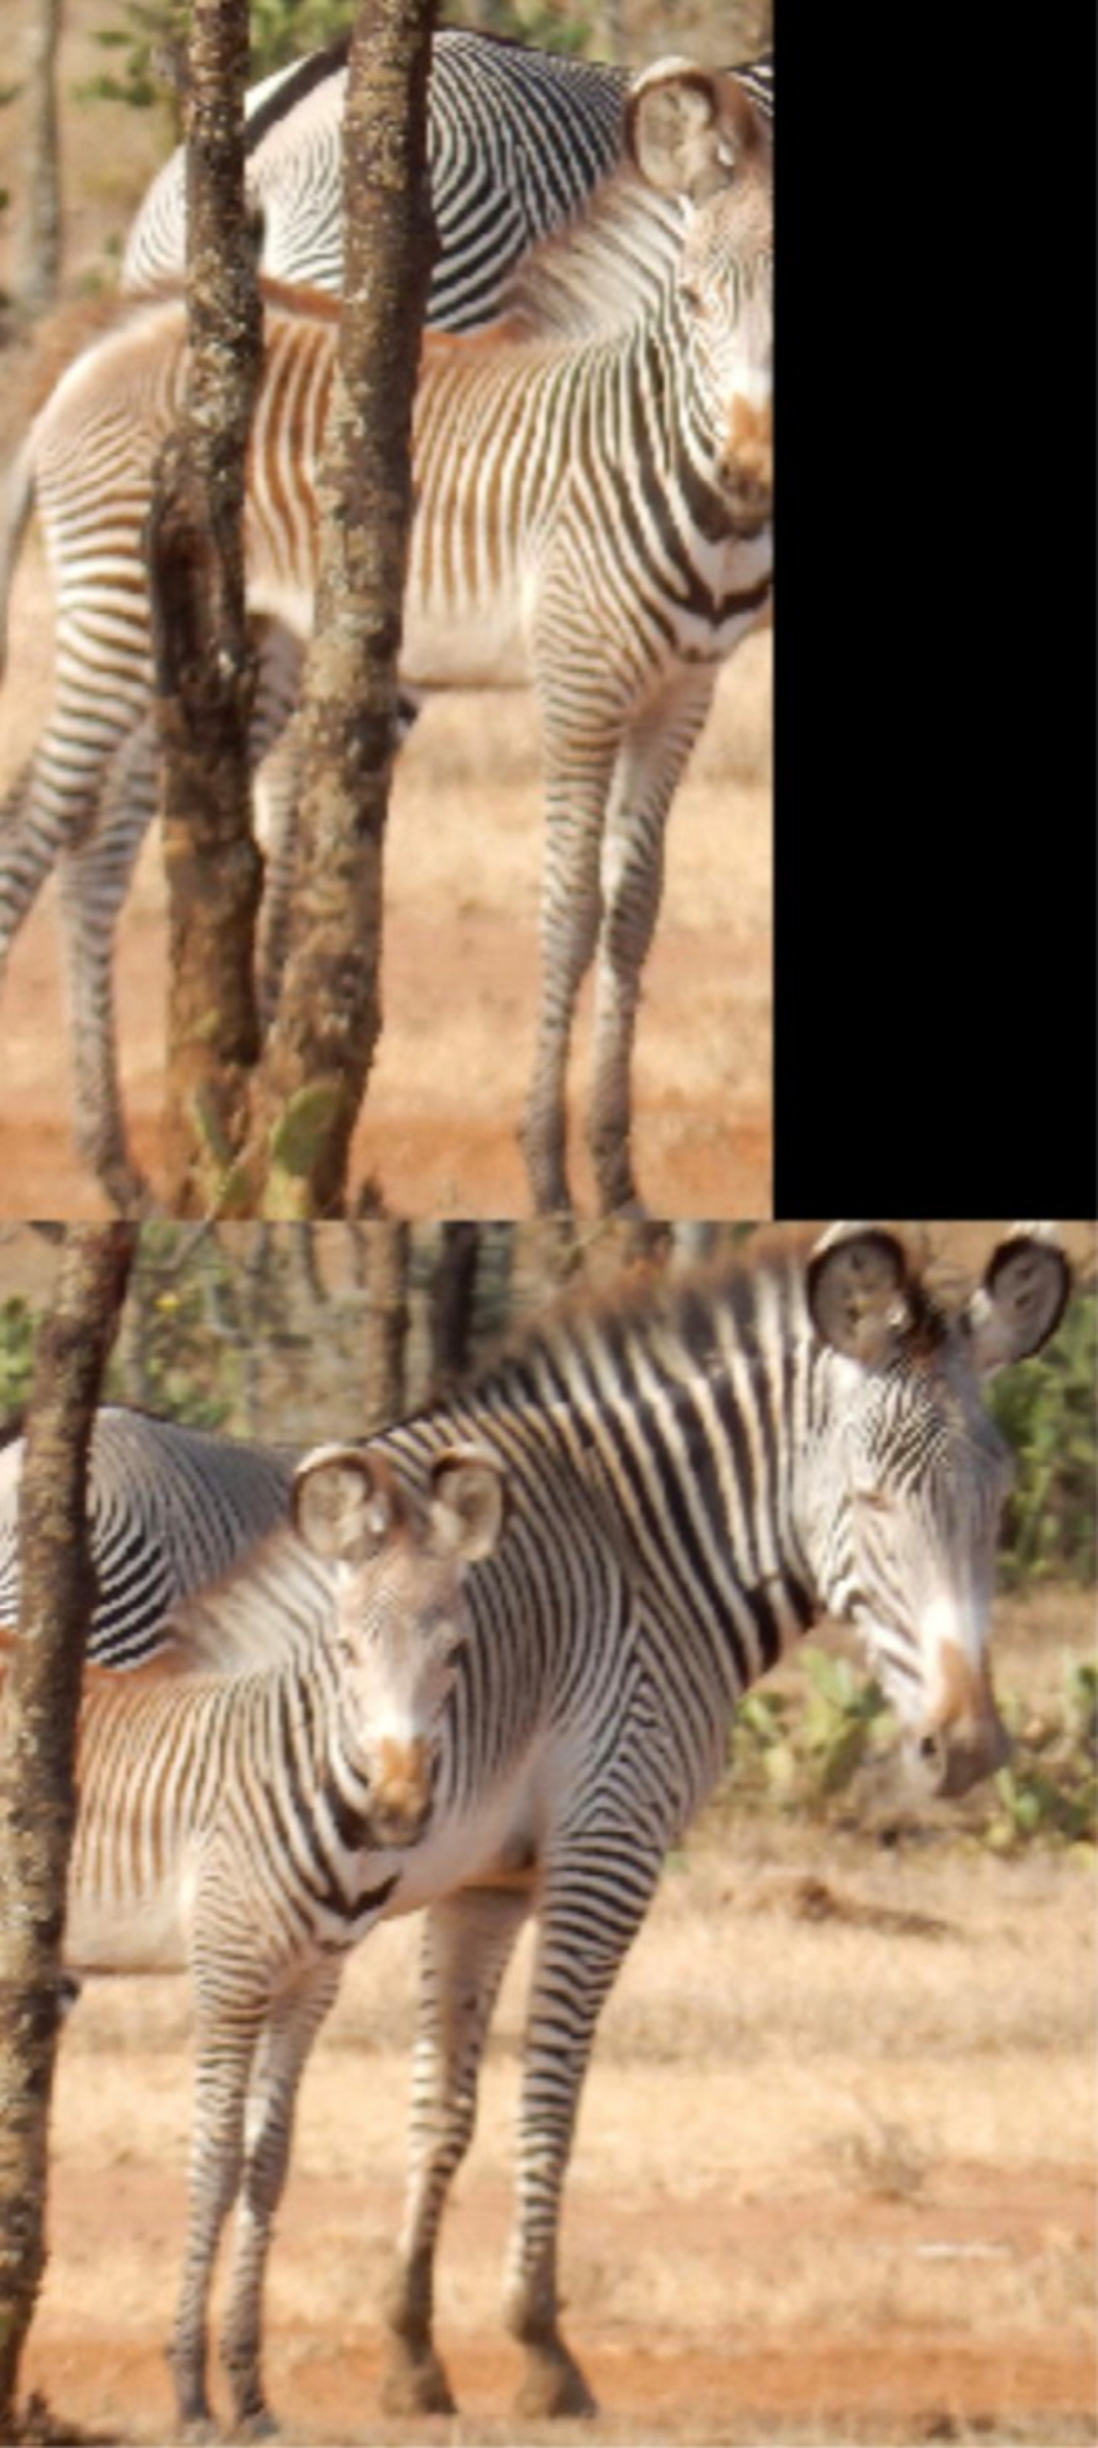
\includegraphics[width=0.214\linewidth]{resources/mother-foal.pdf}
    \end{center}
    \caption{Example images of two types of photobombs taken during the GGR-18.  A typical photobomb (left) happens when the primary animal in the top sighting has matches against itself in the bottom annotation, but it is not the primary sighting in that annotation.  A special case of photobombs, involving splitting mothers and foals (right) in the same image, is particularly challenging to automated ID for herding social species.}
    \label{fig:ca-photobomb}
\end{figure}

A photobomb happens when the primary animal in one annotation matches a non-primary animal in the other annotation.  An example of a photobomb can be seen in Figure~\ref{fig:ca-photobomb} (left), where the primary animals shown in the middle of each annotation are not being appropriately matched (highlighted regions provided by HotSpotter~\cite{crall_hotspotter_2013}).  Photobombs are typical for herding species because animals that are routinely seen together have an increased likelihood of being seen in the background of other images.  Further, a special case of photobombs can also occur between mothers and foals, called ``mother-foal photobombs''.  Young animals often stay close to their mothers for protection~\cite{becker_mother-infant_1990}, which means their annotations can significantly overlap and be accidentally matched.  Figure~\ref{fig:ca-photobomb} (right) gives an example of a mother-foal photobomb for Gr\'evy's Zebra during the Great Gr\'evy's Rally (GGR) 2018.  The demographics for the GGR 2016 census~\cite{berger-wolf_great_2016} report that approximately 10\% of the zebras in the population were infants (0-12 months of age), meaning that these types of photobombs will happen at a non-trivial rate and must be treated as a distinct error mode.

\begin{figure}[!t]
    \begin{center}
        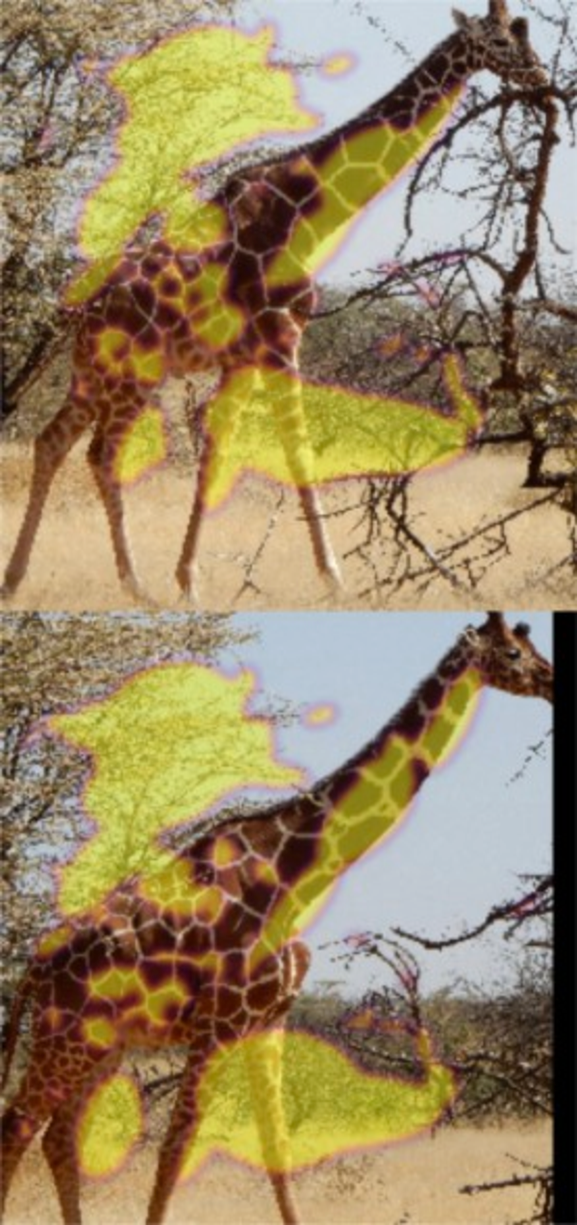
\includegraphics[width=0.53\linewidth]{resources/scenerymatch.pdf}
    \end{center}
    \caption{An example image of a scenery match taken during the GGR-18.  The background scene in this match strongly corresponds while the two primary animals are clearly different individuals.  Semantic segmentation could provide a background mask but would also require novel ground-truth segmentation data for new species.}
    \label{fig:ca-scenery-match}
\end{figure}

Scenery matches, in contrast, are distinct from photobombs because they are based on matching the surrounding background (i.e., trees, shrubs).  One of the most common sources of incidental matching -- especially scenery matches -- is annotations taken within seconds of each other; these ``near-duplicate'' annotations can strongly match because they capture the same scene with significant background overlap.  Scenery matches can also occur when multiple photos are taken from the same spot, although not necessarily on the same day~\cite{beery_recognition_2018}.  By their very nature as stationary cameras, camera traps have a significant potential for scenery matching and must be considered carefully during a photographic census.  Figure~\ref{fig:ca-scenery-match} gives an example of a scenery match for a reticulated giraffe during the GGR 2018 censusing event.  By looking carefully at the giraffe, it is evident that the animals are not the same. However, robust matching is happening by the texture-based algorithm on the background trees and bushes.  The result is that this negative ``different animal'' match will have a strong positive score, complicating our ability to set automatic decision thresholds for pairs in general.

The Census Annotation concept is extended in Chapter~\ref{chapter:ca} to add Census Annotation Regions (CA-R) to avoid incidental matching.  A Census Annotation Region is a smaller, more focused box within a CA that crops out irrelevant background information.  This new bounding box drastically limits the number of overlapping animals and the amount of background seen within the annotation.  The benefit of performing a photographic census on CA-Rs, as we will see, is that it presents highly comparable (and therefore easier) annotation pairs to the automated verifier and vastly reduces the need for human verification to fix bad decisions.

\subsection{Managing the Decision Process: Animal ID Curation}

Now that we have identified the need to filter annotations appropriately and limit the impact of incidental matching, we need to examine the third and final way substantial amounts of human effort are introduced.  Let us consider a fully automated process for building an ID database that uses 1) comparable annotations as input, 2) a ranking algorithm to produce potential matches for each annotation, and 3) a verification algorithm to decide if each match is correct.  The process assigns the same ID to annotation pairs deemed correct and leaves unmatched annotations as different animals.  The immediate question is, ``\textit{is this process sufficient to produce an accurate database of animal IDs?}''  Consider what would happen when the verifier makes a mistake and incorrectly decides that one of the pairs is the same animal when, in fact, it is not.  The IDs for those two animals would be merged, and the population estimate would decrease by one (under-counting).  The second type of error in the ID process occurs in one of two ways: if a verifier or human fails to decide ``same animal'' for an actual match or if the ranking fails to propose the match in the first place.  In this event, the ID for one animal is split across two IDs in the database, and the population estimate would increase by one (over-counting).

The natural way to avoid this problem is to rely on human decision-making instead of the automatic algorithm when there is any chance of error.  Unfortunately, this solution requires many human decisions -- defeating the purpose of automation -- and, as we will see, still does not eliminate all chances of error.  What is needed is an overarching control algorithm that 1) goes beyond the matching pairs that were initially suggested by a ranking algorithm, 2) works to find potential inconsistencies in the match decisions, and 3) resolves issues -- either fixing inconsistencies or reinforcing recent decisions -- by seeking additional information from an algorithm or human.  This algorithm must manage when automated or human decisions are needed to curate a consistent database of animal IDs, and its implementation influences how much human decision-making is required overall.

\subsection{Summary}

In summary, these three challenges are the most significant theoretical barriers to automated photographic censusing.  The underlying problem is that automated computer vision algorithms and even human reviewers make mistakes.  A significant impact of these mistakes -- difficult-to-compare annotations, incidental matching, and matching ambiguities -- is the increased need for human effort to generate a reliable database of IDs.  It is, therefore, appropriate to use human effort as a quantitative metric to compare different censusing configurations.  Therefore, the amount of work done by humans will be the basis for experiments in Chapter~\ref{chapter:ca}.
We now turn our attention to describing the components required to perform a photographic census and discuss the errors they introduce in the final population estimate.  The introduced components are assembled at the end of the chapter to build a new evaluation database for Gr\'evy's zebra IDs.

\section{Components of Animal ID Curation}

The task of large-scale and automated photographic animal censusing is complex.  The above problem description has established that the solution needs multiple components to work successfully as an end-to-end process.  Those components include:

\begin{enumerate}
    \item a \textit{detection pipeline} that finds relevant sightings of animals in images and ensures that all of the resulting annotations are comparable,
    \item a \textit{ranking algorithm} that matches a query annotation against a database of annotations and generates a prioritized ranked list of the most likely pairs that show the same animal,
    \item a \textit{decision management algorithm} that looks for ambiguities and inconsistencies in the database and seeks additional pair decisions from a verification algorithm or human reviewer,
    \item a \textit{verification algorithm} that automatically predicts if two annotations are the same animal or not,
    \item a \textit{human-in-the-loop reviewer} that is tasked by the decision management algorithm to litigate hard pairs when the results of the automated verification algorithm are insufficient, and
    \item a \textit{population estimator} that uses the distribution of sightings and resightings on back-to-back days to estimate the total number of animals in a surveyed population.
\end{enumerate}

\noindent This dissertation addresses the following aspects of this problem: 1) establishing a problem definition, 2) contributing the detection pipeline, 3) proposing a solution to the annotation comparability problem, 4) minimizing the incidental matching problem, 5) building an experimental dataset, 6) configuring, training, building, and validating algorithms and the whole system, and 7) demonstrating its effectiveness on the GGR-16 and GGR-18 censusing events (Chapter~\ref{chapter:censusing}).  The evaluation employs prior and ongoing work for ranking (HotSpotter~\cite{crall_hotspotter_2013} and PIE~\cite{moskvyak_robust_2019}), pair-wise verification (VAMP~\cite{crall_identifying_2017} and PIE~\cite{moskvyak_robust_2019}), and decision-making during ID curation (Graph ID~\cite{crall_identifying_2017} and LCA).  Of particular importance in this work is the first experimental evaluation of the LCA algorithm, demonstrating that it is a successful animal ID curation algorithm.  The remaining discussion in this section will review each of the components listed above and outline the errors that each may introduce in the population estimate.

\subsection{Detection Pipeline}

The detection pipeline, as discussed in Chapter~\ref{chapter:detection}, functions in part to control which annotations are considered for photographic censusing.  By its very design, the output of the detector offers a filtered view to the rest of the photographic censusing procedure because it only allows relevant annotations through to ID.  By operating on the reasonable assumption that the input photographs did not capture all of the individuals in a large population, the reality is that photographic censusing must be designed to estimate how many animals were not seen at all.  When an animal is not cataloged, it means that 1) the animal was not seen by any photographer or 2) the animal was seen by a photographer but the detection pipeline did not create an annotation for it.  Both cases are handled similarly by the population estimator when the chance of a detection error is independent across images and uniformly distributed.  For example, we know that the YOLO localizer can perform poorly on small annotations.  If the analysis considers only Annotations of Interest, this source of error is nullified because useful and small AoIs are rare.  This detail means that the estimator implicitly controls the error introduced by false-negative detections (missed detections) in the final population estimate.

The more worrying case is when the detection pipeline produces an annotation that it should not have let through.  These ``spurious detections'' may have various issues; they could have a poor bounding box, be the wrong species, show an incomparable viewpoint, be too blurry for matching, be occluded in the background, or are otherwise not identifiable.  These annotations are less likely to be successfully matched by an ID ranking algorithm and are therefore more likely added to the animal ID database as singletons.  The result is that false positives from detection can bias the number of animals in the population estimate higher.  In practice, these errors are easy to find by reviewing all of the annotation singleton (or encounter singleton) IDs in the database.  For a little extra human effort to do a final check, this source of error can be mitigated by discarding inappropriate singleton annotations during ID curation.

\subsection{Ranking Algorithm}

After comparable annotations are selected for use in the photographic census, a ranking algorithm is needed to prioritize which pairs of annotations should be reviewed.  The ranking process is a crucial step because an exhaustive review of all quadratic pairs is not feasible.  An established ranking algorithm discussed and used in this dissertation is the HotSpotter~\cite{crall_hotspotter_2013} algorithm, which finds texture-based features on the body of an animal and uses a nearest neighbor search database to create a list of ranked matches.  The algorithm works well as a general retrieval and ranking method and produces numerical scores for each pair in their ranked lists.  These scores, however, are unbounded and do not have a good separation between positive ``same animal'' pairs and negative ``different animal'' pairs, setting up the need for an independent verifier (discussed next).  There are also new types of ranking algorithms, like Pose Invariant Embeddings (PIE)~\cite{moskvyak_robust_2019}, that use deep learning and specialized training methods (i.e., triplet loss) to learn a feature embedding for ID.  These methods are often faster, more flexible, and more accurate compared to their hand-engineered counterparts.  The challenge is that these feature embedding approaches can require significant amounts of ground-truth ID data to train, which presents a problem for photographic censusing as an end-to-end process for new animal species.  The crucial insight with ranking algorithms is that there needs to be an awareness of the capabilities of traditional computer vision algorithms that do not rely on deep learning and an acknowledgment that they are an asset to bootstrapping.

When using ranking algorithms, the most elusive source of error is a ``missed match'' (i.e., a recall failure).  The retrieval rates for a ranking algorithm can be estimated using small databases because they are easier to verify thoroughly.  It becomes challenging, however, to measure this value for larger databases because a ranking algorithm is often needed to build the database in the first place.  Special care is needed, therefore, to ensure that an animal ID database is sufficiently curated with multiple ranking and verification algorithms.  The second type of error from a matching failure is a ``spurious match'', which is most often caused by incidental matching.  As we will see, the use of Census Annotation Regions and a decision management algorithm helps to drive this rate towards zero during ID curation.  A final consideration is that some animals may be photographed multiple times at the same general time and place -- considered a single ``encounter'' of that animal -- and the ranking algorithm needs to support both short-term (intra-encounter) and long-term (inter-encounter) matching.  The general expectation is that the rate of accurate matching within an encounter is expected to be higher than between encounters.

\subsection{Decision Management Algorithm}

The management algorithm leveraged in most of this work is called the Graph ID algorithm by Crall~\cite{crall_identifying_2017}.  The Graph ID algorithm is a linear curation process that enforces an explicit level of decision redundancy within animal IDs (positive redundancy) and between animal IDs (negative redundancy).  The Graph ID algorithm is easy to understand but has the downside that it is too aggressive at enforcing consistency.  For example, when an inconsistency is found, the automated verifier is disabled, and manual decision-making by humans is needed to find and fix the issue.  Furthermore, the algorithm only uses automated verifiers up to a pre-defined threshold (generally a false-positive rate of 1\%).  In practice, this means that most of the ID verification decisions are performed by humans.  A second decision management algorithm called LCA (Local Clusters and their Alternatives) discards the need for explicit redundancy and instead measures an animal ID's stability relative to an alternative clustering of annotations.  LCA intentionally delays human effort as long as possible and uses an automated verifier more effectively by weighting its decisions into a probabilistic vote (compared to a binary decision threshold with Graph ID).  The result is that LCA requires much less human effort to resolve inconsistencies and curate the database of animal IDs.

The goal of photographic censusing is to produce a consistent database of animal IDs such that no additional splits or merges need to occur.  However, it is significantly more likely to have a silent merge case between the two possible cases because it cannot be identified without some positive signal from a ranking algorithm.  On the other hand, missed splits can be identified more easily by analyzing the state of the database and ensuring each animal ID is sufficiently reviewed. Thus, any bias introduced in the final population estimate is ultimately a matter of how comprehensively the algorithm reinforces the animal IDs, and by default, the estimate should be treated as an upper bound.  For example, the decision management algorithm can include a method to ``densify'' small animal IDs with extra decisions, which helps identify the need for potential ID splits.

\subsection{Verification Algorithm}

The purpose of an automated verifier is to review pairs suggested by the decision management algorithm, and it functions as an accurate stand-in for a human reviewer.  The Verification Algorithm for Match Probabilities (VAMP)~\cite{crall_identifying_2017} approach was the first verification algorithm developed for use in automated photographic censusing\footnote{The Graph ID algorithm, using the detection pipeline to find comparable annotations along with HotSpotter as its ranking algorithm and VAMP as its verifier, was used as the original algorithmic tool-chain for the Great Gr\'evy's Rally (GGR), as discussed in Chapter~\ref{chapter:censusing}}.  VAMP is implemented as a random forest classifier that uses hand-engineered features to compare two annotations and produces a probabilistic decision of ``same animal'' or ``different animals''.  The algorithm is noticeably fast and, while it does require ID training data, it can be trained from a relatively small database due to a mining procedure.  The second type of verification algorithm can be constructed with the same triplet-loss embedding networks used for ranking.  Since the embedding for two annotations is trained to be directly compared in embedding space, a distance between two annotations can also be calculated and used for verification.  Like with ranking, however, the PIE algorithm needs an extensive database to train effectively; VAMP, in contrast, can work as a bootstrapable verification algorithm before a critical mass of ground-truth IDs can be collected.

The automated verifier's accuracy -- and the separability of its scores -- directly affects how automated photographic censusing can be. Furthermore, any error this component introduces ends up translating directly into the need for more human effort to find and fix inconsistencies in the animal ID database, and its failures should have a minimal impact on the final estimate.

\subsection{Human-in-the-Loop Reviewer}

Likewise, human reviewers are not perfect and make mistakes.  Each mistake made by a human requires the decision management algorithm to request more overall work to find and fix the database issues it causes, just as when the automated verifier makes an incorrect decision.  Making the matter worse, the pairs given to humans for review are not consistent in their difficulty.  Some pairs are easy to compare and contrast and, as a result, are faster to review. However, when a pair is complex or shows two annotations that are borderline comparable, then the human reviewer spends significantly more time making a decision.  Since our goal is to reduce overall human effort, the most obvious way to achieve this is to automate decision-making with verification algorithms.  However, an additional way to reduce effort is to focus on annotation pairs that are easy and fast for humans to review.  The error introduced by human reviewers, like the automated verifier, also converts to more overall work during ID curation.  This feature of photographic censusing is convenient because it suggests that a comprehensive pairwise review attenuates the effects of human mistakes in the final population estimate.

It is important to note that if humans cannot accurately verify the results of a ranking algorithm, then that algorithm or species is not compatible with photographic censusing.  Further, a person must be able to manually filter out annotations that are of undesired species, of incompatible viewpoints, of incomprehensible quality, and are ultimately \textit{incomparable} because all of these are the actions needed to bootstrap the detection pipeline and curate IDs in the first place.

\subsection{Population Size Estimator}

Lastly, we need to highlight that an animal ID database does not provide a population estimate by itself.  The animal population is likely open, and the number of known animals in the database does not tell us anything about many \textit{unknown} animals still remain in the population.  Put simply, how do we know if an ID database is complete and has 100\% coverage?  Any animal database for an open population will have the possibility of animals that have never been cataloged.  What is needed is a way to use a curated and consistent animal ID database to estimate the total number of animals in the population.  The sampling method used by sight-resight studies, the Lincoln-Petersen estimator~\cite{petersen_valuation_1911}, is a relatively simple ratio calculation.  Its simplicity has made it a popular method by ecologists for baseline studies, and it is used for photographic censusing because it allows for more direct comparisons with historical estimates.  One advantage of large-scale photographic censusing is that it is designed to be a drop-in replacement for past, more limited surveys.

The Lincoln-Petersen (LP) estimator can be extended for our use with machine learning algorithms.  One of the advantages of machine learning algorithms is that their error rates can be experimentally measured during validation, and the effects of automatic failures in the final population estimate can be considered.  The various sources of error discussed in this chapter are limited to specific scenarios around missing and making spurious detections, failing to recall matches during ID ranking, and incidentally matching annotations.  An updated version of the LP estimator is proposed in the next section that adds new error terms and discusses their impact on the final population estimate.

\section{Automated Lincoln-Petersen Estimator} \label{sec:ca-math}

While the Lincoln-Petersen estimator is well established and has been expanded since its formation, it has not been amended to add explicit terms for automated machine learning errors.  This section provides a mathematical framework for estimating an animal population using the automated tools and concepts proposed above for photographic censusing.  To provide a quick overview: the Lincoln-Petersen estimator and confidence interval (CI) can be modified to add four high-level error rates: missed detections, spurious detections, missed matching, and spurious matching.  The estimated rate of missing a match (recall failure) and incorrectly matching two animals together (incidental matching) impact the population estimate the most. In contrast, the rate of missing detections has the most significant impact on confidence interval.  One of the convenient takeaways is that aggressive annotation filtering (artificially high detection miss rate) should have little impact on the actual predicted estimate.  Further, spurious detections are easy to identify and eliminate during ID curation, ideally a rate of zero in practice by reviewing singletons.  Likewise, when the ranking algorithm fails to match at a higher rate than it makes spurious matches, then the population estimate will, as expected, be biased high, and the CI will grow.  For readers who wish to skip the details of its derivation, the final resulting Equation~\ref{eq:final} is used in Chapter~\ref{chapter:censusing} to produce a population estimate for Gr\'evy's zebra in Kenya.  Section~\ref{sec:gzcd} continues the discussion by describing an evaluation dataset for Census Annotations in Chapter~\ref{chapter:ca}.

\subsection{Assumptions} \label{sec:assumptions}

The population estimate applies to a fixed time window, where images of animals are taken on day 1 and again for a subsequent, consecutive day 2.  The number of animals sighted on each day and the number sighted on {\it both} days (resights) provides the foundation for a sight-resight study. However, for this process to work accurately, it must rely on a set of assumptions about the data collection and underlying animal detection and identification algorithms.

\begin{enumerate}
    \item \textbf{Equal Sightability} - The animal population is considered closed (geographically and demographically) during the two days of the census; no significant immigrations, emigrations, births, or deaths should occur, and the actual number of animals is expected not to fluctuate during the survey period~\cite{jolly_problem_1983}.
    \item \textbf{Passive Influence} - Any given animal, or any given group of animals, is equally likely to be sighted throughout any given day, and across both days, of the census; seeing an animal does not affect its likelihood of being seen later that day or resighted on day 2.
    \item \textbf{Encounter Coverage} - When an animal or a group of animals is encountered, {\it exactly one} comparable annotation is captured by the photographer(s); this assumption requires that if a photographer encounters an animal, then it cannot be skipped over; another way to phrase this is matching within an encounter of comparable sightings is trivial and assumed to have perfect recall.
    \item \textbf{Population Coverage} - The total number of animal sightings on day 1, day 2, and the number of resightings on each day and between both days are non-trivial (i.e., not zero or close to zero); the assumption specifies that the scale of data collection is sufficiently large and that the ID database offers meaningful and uniform coverage over the animal population.
    \item \textbf{Comparable Sightings} - The animal species must be comparable; any given pair of annotations must be verifiable by a human (with high confidence and accuracy) to be either a) same individual or b) different individuals.
    \item \textbf{Match Retrieval} - The probability of the ranking algorithm failing to retrieve (recall) a correct ``same animal'' match between encounters is assumed to be non-zero but also constant throughout the census, regardless of the size of the underlying animal ID database.
\end{enumerate}

\noindent These assumptions should be realized through a careful design of the data collection procedure, which will be the focus of Chapter~\ref{chapter:censusing} and \textit{photographic censusing rallies}.  For example, the data collection process should ensure that the census area is comprehensive and covers the known regions that contain the resident population.

\subsection{Animal Detection}

A photographic census is a process where images are captured in a two-day collection and processed by an automated system.  The first step of this automated processing is detection, and it places a box and species label around each animal in the collected images.  Let $\alpha \in \{1, 2\}$ signify either the $1^{\text{st}}$ or $2^{\text{nd}}$ day of the census, where each has a set of images that can be treated independently.  For each day, there are the following:

\begin{align*}
    \begin{split}
        s_{\alpha} &\textnormal{\hspace{0.2cm}---\hspace{0.2cm}} \text{total number of animal sightings of the desired species} \\
        &\hspace{0.82cm} \text{captured by the images} \\
        s^{\prime}_{\alpha} &\textnormal{\hspace{0.2cm}---\hspace{0.2cm}} \text{total number of {\it comparable} animals within $s_{\alpha}$, where $s^{\prime}_{\alpha} \leq s_{\alpha}$} \\
        d_{\alpha} &\textnormal{\hspace{0.2cm}---\hspace{0.2cm}} \text{total number of animal detections of the desired} \\
        &\hspace{0.82cm} \text{species derived from the images}
    \end{split}
\end{align*}

\noindent Since we only care about the animal sightings that are visually comparable, we can set the expected number of annotations $a_{\alpha}$ to be:

\begin{align} \label{eq:detection}
    \begin{split}
        a_{\alpha} &= (1 - p_{dm}(\theta))*s^{\prime}_{\alpha} + p_{ds}(\theta)*d_{\alpha} \\
        \text{where} \hspace{1cm} & \\
        p_{dm}(\theta) &\textnormal{\hspace{0.2cm}---\hspace{0.2cm}} \text{probability of missing an animal detection, given $\theta$} \\
        p_{ds}(\theta) &\textnormal{\hspace{0.2cm}---\hspace{0.2cm}} \text{probability of adding a spurious, incomparable detection, given $\theta$} \\
        \theta &\textnormal{\hspace{0.2cm}---\hspace{0.2cm}} \text{detection parameter controlling the level of annotation filtering}
    \end{split}
\end{align}

\noindent The detection probabilities above aggregate the chances of making a detection error into a single value regardless of the reason.  The reasons for making a detection error vary and include factors like qualitative properties of the image (e.g., illumination, sharpness) and semantic properties (e.g., an animal is truncated, occluded, or of a commonly confused, visually similar species) but can be estimated for an entire dataset.  The variable $\theta$ represents the collection of parameters that control the filtering level applied on the annotations passed to ID.  These parameters influence the error rates of the detector because -- for example -- in focus, clear, un-occluded, and well-lit annotations are easier to find, and the system will make more mistakes as poorer annotations are included.  Furthermore, the error rates must use comparable annotations as the frame of reference for correct detections.

\subsection{Individual Identification on Day 1 and 2}

Provided with the number of {\it comparable} annotations $a_{\alpha}$ for day $\alpha$, we need to estimate the number of unique individuals $n_{\alpha}$ that was sighted on that day.  The number of individuals $n_{\alpha} \leq a_{\alpha}$ but, in general, we expect $n_{\alpha} << a_{\alpha}$ to be the case for a large-scale photographic census with sufficient coverage.  An animal's average number of resightings is expected to be non-trivial and is further guaranteed by assumption 4.  Therefore we need a general matching algorithm that can prioritize the potential $\binom{a_{\alpha}}{2}$ pairs of annotations for analysis and decide if the annotations are either a) the same individual or b) different individuals.  All pairwise decisions are guaranteed to be decidable through assumption 5 because an incomparable pair cannot exist.  Furthermore, any incomparable pair that is found needs to be manually reviewed to discard the offending annotation(s).  This manual review means that each of the decisions has a chance of being decided correctly or incorrectly.  An incorrect match could happen by either missing a match (failing to associate two annotations of the same individual correctly) or making a spurious match (failing to distinguish two annotations of a different individual correctly).

In practice, however, it can be too complex to estimate the pairwise error probabilities of missing a given match.  The reasons for this are varied and are often a consequence of the implementation details of the matching algorithm.  For example, the na\"ive search space for the match pairs is $O(n^2)$, but a given matching algorithm may choose to perform an approximated search of this space on visually similar neighbors, meaning not all pairs will be explicitly reviewed.  Thus, there is a probability that the matching algorithm may fail to include a correct pair in the decision process. However, this probability is complex and may not be the only factor in missing a particular correct match. Therefore, we would prefer to contextualize the matching problem not in terms of a {\it pairwise} probability of matching failure but rather in terms of a {\it global} probability of matching failure, averaging the various effects and relying on a general performance validation of the algorithm.  Further, we expect that these rates of ID failure are constant and do not depend on the size of the search database (assumption 6). Therefore, we set:

\begin{align} \label{eq:matching}
    \begin{split}
        n_{\alpha} &= n^{\prime}_{\alpha} * (1 + p_{mm}(\theta) - p_{ms}(\theta)) \\
        \text{where} \hspace{1cm} & \\
        n^{\prime}_{\alpha} &\textnormal{\hspace{0.2cm}---\hspace{0.2cm}} \text{actual number of individuals captured by $a_{\alpha}$} \\
        p_{mm}(\theta) &\textnormal{\hspace{0.2cm}---\hspace{0.2cm}} \text{probability of missing a match, given $\theta$} \\
        p_{ms}(\theta) &\textnormal{\hspace{0.2cm}---\hspace{0.2cm}} \text{probability of making a spurious match, given $\theta$}
    \end{split}
\end{align}

\noindent We would prefer, however, to define $n^{\prime}_{\alpha}$ in terms of $a_{\alpha}$.  Let us assume that there exists some $k_{\alpha} \in \R^{+}$ which represents the average number of annotations per individual on day $\alpha$, where:

\begin{align} \label{eq:lemma_start}
    \begin{split}
        n^{\prime}_{\alpha} &= \left\lfloor \frac{1}{k_{\alpha}} * a_{\alpha} \right\rfloor
    \end{split}
\end{align}

\noindent Assumption 3 guarantees that when an individual photographer (or a group of photographers in the same survey vehicle) encounters a single animal (or a group of animals), then the photographer(s) act in unison as a single oracle.  The ``photographic oracle'' is expected to capture \textit{exactly one} comparable annotation for \textit{every} individual in the encounter, and there will be multiple independent oracles during a photographic census.  This assumption is exceedingly strong about $a_{\alpha}$ and places an unrealistic expectation on the level of skill and coordination between the photographers.  Let us consider a relaxation for the moment where more than one annotation for an animal was allowed to be collected but still required for every animal.  This second requirement becomes easier to meet when there are multiple photographers in the same survey vehicle.  This condition also would mean multiple annotations were taken at the same general time and place for the same animal.  Let $a^{\prime}_{\alpha}$ represent the total number of comparable annotations that were collected before any sort of de-duplication is performed for each encounter, where $a_{\alpha} \leq a^{\prime}_{\alpha}$.

The difference between $a_{\alpha}$ and $a^{\prime}_{\alpha}$ is that the only way to get a repeat annotation of an individual with $a_{\alpha}$ is by photographing it at a different encounter.  In other words, the value for $k_{\alpha}$ is equal to the average number of encounters an animal is seen on day $\alpha$ of the census.  Each encounter is limited to a fixed spatio-temporal context with a unique duration, interval, and geographic area; the number of individuals seen during each encounter will also vary.  Each encounter, however, is a specific event and occurs independently of all other encounters.  Assumptions 1 and 2 guarantee that the movement and behavior of the animals are truly independent of the ongoings of the census and that the chance of sightings is uniform.  We can also reason that the chance a given group of animals is encountered by two oracles simultaneously is practically zero. However, in any such event, the oracles are simply merged for that single encounter.  Since there is no real-time coordination between photographic oracles (which is allowed to encourage better coverage of the survey area), then the process of any oracle encountering any given animal can be modeled as a Poisson random process.  This process has an expected value $k^{\prime}_{\alpha}$ for the average number of annotations per individual and is conditioned on day $\alpha$ because the averages can differ day-by-day.

\newpage

\noindent Thus, the expected number of annotations per animal is defined as:

\begin{align} \label{eq:lemma}
    \begin{split}
        \left\lfloor k^{\prime}_{\alpha} * n^{\prime}_{\alpha} \right\rfloor  &= a^{\prime}_{\alpha} \\
        n^{\prime}_{\alpha} &= \left\lfloor \frac{1}{k^{\prime}_{\alpha}} * a^{\prime}_{\alpha} \right\rfloor \\
        \text{where} \hspace{1cm} & \\
        k^{\prime}_{\alpha} &\in \R^{+} \\
        \text{and} \hspace{1cm} & \\
        k^{\prime}_{\alpha} &\geq k_{\alpha}
    \end{split}
\end{align}

\noindent What is needed is to bridge the gap between Equations~\eqref{eq:lemma_start} and ~\eqref{eq:lemma} by substituting $k^{\prime}_{\alpha}$ and $a^{\prime}_{\alpha}$ with their de-duplicated counterparts.  In order to do this, the data collection procedure needs to ensure that 1) the average number of annotations per animal is uniform within an encounter and 2) that the average number of annotations per animal is uniform throughout the day.  A real-world example of collection bias is when an encountered group of animals contains an infant.  We can reasonably expect that the number of photographs for an infant will be biased arbitrarily high compared to an adult in the same group.  The reason is simple: baby animals are cute.  This effect can also be seen when an individual photographer encounters a new species and wants to capture many images of it.  Another anticipated source of bias is that the chance of taking a picture for a given individual is not consistent throughout the day, in a phenomenon called ``photographer fatigue''.  An initial excitement defines this fatigue at the start of the census rally, resulting in more images taken during the first couple of encounters.  As the day progresses, the photographer becomes tired, and the average number of annotations per animal decreases.

Three important factors can help control for these kinds of biases.  The first is to have multiple photographers within the same survey vehicle.  Having multiple cameras in a car will average out the effect of a single photographer and make their unified photographic oracle more uniform in its behavior.  The second is that the photographers should be trained specifically on these two effects (excitement and fatigue) and be encouraged to act consistently throughout the day.  The third is that the encounter should contain at least one comparable annotation for each encountered animal regardless of its underlying distribution of duplicate sightings.  Assumption 3 specifies that the recall rate of ID ranking is 100\% within an encounter, which is reasonable because a much smaller context is being compared for duplicates (not across the entire census, but just at one time and space). Furthermore, the chance of missing a match or making a spurious match should be the same as the chance of making an error between encounters,  meaning the terms can be safely substituted.  Combining Equations~\eqref{eq:detection},~\eqref{eq:matching}, and~\eqref{eq:lemma_start} gives us the estimated number of individuals on day $\alpha$ as a function of the number of annotations:

\begin{align}
    \label{eq:names}
    \begin{split}
        n_{\alpha} &= n^{\prime}_{\alpha} * (1 + p_{mm}(\theta) - p_{ms}(\theta)) \\
        &= \left\lfloor \frac{1}{k_{\alpha}} * a_{\alpha} \right\rfloor * (1 + p_{mm}(\theta) - p_{ms}(\theta)) \\
        &= \left\lfloor \frac{1}{k_{\alpha}} * \lbrack (1 - p_{dm}(\theta))*s^{\prime}_{\alpha} + p_{ds}(\theta)*d_{\alpha} \rbrack * (1 + p_{mm}(\theta) - p_{ms}(\theta)) \right\rfloor
    \end{split}
\end{align}

\noindent Equation \eqref{eq:names} relies on several error probabilities that can be estimated for the various automated components. Notably, none of them are conditioned on $\alpha$, implying that the performance of a given algorithm does not depend on exactly when an image was captured.  We can safely assume this to be the case because the rally has fixed start and end times and (at least for the GZGC and GGR) occurs during the same daytime hours.  The equation does, unfortunately, rely on knowing the actual number for $s^{\prime}_{\alpha}$.  Humans could manually review the images to obtain their exact values, but a random sampling of all collected should be sufficient to estimate it.  Given a reviewed subset (e.g., 10\%) of the complete set of comparable sightings ($s^{\prime}_{\alpha}$ annotations) and the total number of detections ($d_{\alpha}$), each of the error probabilities can be estimated.  Furthermore, the estimated rate of missing a detection can also be re-parameterized on $d_{\alpha}$ so that the detector error rates are directly comparable and are calculated as a function of the detector's output.  In other words, for each correct bounding box that is predicted, we can calculate the rate a second box for a missed comparable annotation should have been predicted (on average). Thus, the estimated miss detection rate can be re-defined such that:

\begin{align} \label{eq:substitution}
    \begin{split}
        (1 - p_{dm}(\theta))*s^{\prime}_{\alpha} \approx (1 - \hat{p}_{dm}(\theta))*d_{\alpha}
    \end{split}
\end{align}

\noindent Reformulating Equation \eqref{eq:names} with the respective substitutions for the estimated error probabilities, and using Equation \eqref{eq:substitution}, results in:

\begin{align} \label{eq:individuals}
    \begin{split}
        n_{\alpha} &= \left\lfloor \frac{1}{k_{\alpha}} * \lbrack (1 - p_{dm}(\theta))*s^{\prime}_{\alpha} + p_{ds}(\theta)*d_{\alpha}\rbrack * (1 + p_{mm}(\theta) - p_{ms}(\theta)) \right\rfloor  \\
        &\approx \left\lfloor \frac{d_{\alpha}}{\hat{k}_{\alpha}} * (1 - \hat{p}_{dm}(\theta) + \hat{p}_{ds}(\theta)) * (1 + \hat{p}_{mm}(\theta) - \hat{p}_{ms}(\theta)) \right\rfloor \\
        &\approx \left\lfloor \hat{n}_{\alpha} * (1 - \hat{p}_{dm}(\theta) + \hat{p}_{ds}(\theta)) * (1 + \hat{p}_{mm}(\theta) - \hat{p}_{ms}(\theta)) \right\rfloor \\
        \text{where} \hspace{1cm} & \\
        \hat{n}_{\alpha} &\textnormal{\hspace{0.2cm}---\hspace{0.2cm}} \text{number of animals in the ID database seen on day $\alpha$}
    \end{split}
\end{align}

\subsection{Individual Identification Between Days 1 and 2}

Given the number of individuals seen on day 1 and day 2, represented by $n_1$ and $n_2$ from Equation \eqref{eq:individuals}, we now need to model the number of individuals $n_{B}$ that were seen on {\it both} days.  Following the same logic as Equation~\eqref{eq:names}, we let:

\begin{align} \label{eq:both}
    \begin{split}
        n_{B} &= n^{\prime}_{B} * (1 + p_{mm}(\theta) - p_{ms}(\theta)) \\
        &= \left\lfloor \frac{1}{k_{B}} * a_{B} \right\rfloor * (1 + p_{mm}(\theta) - p_{ms}(\theta))
    \end{split}
\end{align}

We need to recall Equation \eqref{eq:detection}, however, to consider the total number of annotations that are involved.  Before, when considering only one day at a time, we could estimate the probability of missing the detection for a given day as a single event.  The value for $a_{B}$, however, is based on a joint probability of a successful detection (and successful comparable decision) in both day 1 {\it and} in day 2.  Luckily, these joint probabilities are independent and can be combined.  Furthermore, it is incredibly unlikely to match spurious detections across days (regardless of $\theta$) and it can be assumed that $p_{ds}(\theta) = 0$ for resightings.  The value for $a_{B}$ is therefore defined as:

\begin{align} \label{eq:both_a}
    \begin{split}
        a_{B} &= (s^{\prime}_{1} + s^{\prime}_{2}) * Prob(\text{detected on day 1} \cap \text{detected on day 2}) \\
        &= (s^{\prime}_{1} + s^{\prime}_{2}) * Prob(\text{detected on day 1}) * Prob(\text{detected on day 2}) \\
        &= (s^{\prime}_{1} + s^{\prime}_{2}) * (1 - p_{dm}(\theta))^2
    \end{split}
\end{align}

\noindent Substituting Equation \eqref{eq:both_a} into Equation \eqref{eq:both}, and applying the same substitutions used in \eqref{eq:names}, results in:

\begin{align} \label{eq:individuals_both}
    \begin{split}
        n_{B} &= \left\lfloor \frac{1}{k_{B}} * a_{B} \right\rfloor * (1 + p_{mm}(\theta) - p_{ms}(\theta)) \\
        &\approx \left\lfloor \frac{d_{1} + d_{2}}{\hat{k}_{B}} * (1 - \hat{p}_{dm}(\theta))^2 * (1 + \hat{p}_{mm}(\theta) - \hat{p}_{ms}(\theta)) \right\rfloor \\
        &\approx \left\lfloor \hat{n}_{B} * (1 - \hat{p}_{dm}(\theta))^2 * (1 + \hat{p}_{mm}(\theta) - \hat{p}_{ms}(\theta)) \right\rfloor \\
        \text{where} \hspace{1cm} & \\
        \hat{n}_{B} &\textnormal{\hspace{0.2cm}---\hspace{0.2cm}} \text{number of animals in the ID database seen on both days}
    \end{split}
\end{align}

\subsection{Animal Population Estimation}

We now have the estimated total number of individuals seen on day 1 ($n_{1}$), day 2 ($n_{1}$), and the number of individuals sighted on both days ($n_{B}$).  Let $n_{T} \in \Z^{+}$ be the actual total number of individuals in the animal population.  We would also like to estimate $n_{T}$ as well, given the ratio of animals that were resighted ($n_{B}$) by calculating its most likely value.  The likelihood function for $n_{T}$ is sampled from a hypergeometric distribution and, since we are sampling (without replacement) from a fixed pool of individuals, is defined as:

\begin{align}
    \begin{split}
        L(n_{T} | n_{B}) &= \ddfrac{\binom{n_{1}}{n_{B}} * \binom{n_{T} - n_{1}}{n_{2} - n_{B}}}{\binom{n_{T}}{n_{2}}}
    \end{split}
\end{align}

\noindent To find the most likely population estimate $\underset{n_{T}}{\mathrm{argmax}}\hspace{0.2cm} L(n_{T} | N_{B})$ we must measure the increase in likelihood from $n_{T-1}$ to $n_{T}$ since we cannot integrate it directly as a non-continuous integer value.  We must instead maximize the ratio of likelihoods as:

\begin{align}
    \begin{split}
        \frac{L(n_{T} | n_{B})}{L(n_{T} - 1 | n_{B})} &= \ddfrac{\frac{\binom{n_{1}}{n_{B}} * \binom{n_{T} - n_{1}}{n_{2} - n_{B}}}{\binom{n_{T}}{n_{2}}}}{\frac{\binom{n_{1}}{n_{B}} * \binom{n_{T} - n_{1} - 1}{n_{2} - n_{B}}}{\binom{n_{T} - 1}{n_{2}}}} \\
        &= \ddfrac{(n_{T} - n_{1})*(n_{T} - n_{2})}{n_{T} * (n_{T} - n_{1} - n_{2} + n_{B})}
    \end{split}
\end{align}

\noindent The above ratio exceeds 1 if and only if

\begin{align}
    \begin{split}
        n_{T} * (n_{T} - n_{1} - n_{2} + n_{B}) &< (n_{T} - n_{1})*(n_{T} - n_{2}) \\
        n_{T} &< \ddfrac{n_{1}n_{2}}{n_{B}}
    \end{split}
\end{align}

\noindent Therefore, the maximum likelihood for the population estimate is:

\begin{align} \label{eq:census}
    \begin{split}
        n_{T} = \left\lfloor \ddfrac{n_{1}*n_{2}}{n_{B}} \right\rfloor
    \end{split}
\end{align}

\noindent Equation \eqref{eq:census} forms the statistical basis of the Lincoln-Petersen~\cite{petersen_valuation_1911} estimator when it is assumed that $n_{T}$ is sampled from a uniform prior distribution (Assumption 1).  Furthermore, a confidence interval (CI) can be added to the estimator using the appropriate Weld method, as derived by~\cite{seber_estimation_1982} and~\cite{chapman_fallow_1975}:

\begin{align} \label{eq:mean_var}
    \begin{split}
        n_{LP} &= \mu_{LP} \pm z_{\alpha/2} * \sigma_{LP} \\
        \text{where} \hspace{1cm} & \\
        \mu_{LP} &= n_{T} = \left\lfloor \ddfrac{n_{1}*n_{2}}{n_{B}} \right\rfloor \\
        \text{and} \hspace{1cm} & \\
        \sigma_{LP} &= \sqrt{\ddfrac{n_{1}*n_{2}*(n_{1} - n_{B})*(n_{2} - n_{B})}{n^3_{B}}}
    \end{split}
\end{align}

\noindent The final Lincoln-Petersen population estimate $n_{LP}$ is a value with a likelihood range\footnote{The $\alpha$ term here is overloaded in our notation and does not refer to the day $\alpha$, but rather a proportion of likelihood for the estimate falling outside of the CI.}.  For a confidence interval of $95\%$, we set $z_{\alpha/2} = 1.96$.

\newpage

\subsection{Population Estimate Mean}

Combining Equations \eqref{eq:individuals} and \eqref{eq:individuals_both} with \eqref{eq:mean_var} for the population estimate mean $\mu_{LP}$:

\begin{align}
    \begin{split}
        \mu_{LP} &= \left\lfloor \ddfrac{n_{1}*n_{2}}{n_{B}} \right\rfloor \\
        &\approx \left\lfloor \ddfrac{\hat{n}_{1} * \hat{n}_{2} * (1 - \hat{p}_{dm}(\theta) + \hat{p}_{ds}(\theta))^2 * (1 + \hat{p}_{mm}(\theta) - \hat{p}_{ms}(\theta))}{\hat{n}_{B} * (1 - \hat{p}_{dm}(\theta))^2} \right\rfloor \\
        &\approx \left\lfloor \ddfrac{\hat{n}_{1} * \hat{n}_{2}}{\hat{n}_{B}} \right\rfloor * \ddfrac{(1 - \hat{p}_{dm}(\theta) + \hat{p}_{ds}(\theta))^2 * (1 + \hat{p}_{mm}(\theta) - \hat{p}_{ms}(\theta))}{(1 - \hat{p}_{dm}(\theta))^2} \\
        &\approx \hat{\mu}_{LP} * \ddfrac{(1 - \hat{p}_{dm}(\theta) + \hat{p}_{ds}(\theta))^2 * (1 + \hat{p}_{mm}(\theta) - \hat{p}_{ms}(\theta))}{(1 - \hat{p}_{dm}(\theta))^2}
    \end{split}
\end{align}

\noindent This implies that the final Lincoln-Petersen estimate $\mu_{LP}$ is approximated by the estimate $\hat{\mu}_{LP}$ as calculated directly from the number of animals and resightings in the animal ID database.  In practice, the parameters for $\theta$ can be selected such that the chance of adding a spurious, {\it comparable} detection to the census is low, with the ID curation process also ensuring that the chance is functionally zero by requiring a final review of all singletons for irrelevant or incomparable annotations.  As a result, if the animal IDs in the database are comprised of only relevant and comparable annotations, then $\hat{p}_{ds}(\theta) = 0$. Thus, the ratio between the final and calculated estimates is:

\begin{align}
    \begin{split}
        \ddfrac{\mu_{LP}}{\hat{\mu}_{LP}} &\approx 1 + \hat{p}_{mm}(\theta) - \hat{p}_{ms}(\theta)
    \end{split}
\end{align}

\noindent and indicates that matching errors mainly impact the final population estimate.  This derivation is encouraging for our desire to do annotation filtering because it implies that focusing on comparability and automated curation has less impact on the accuracy of the population estimate.  When the rate of spurious detections is zero, the bias from unmatched singletons to push the population estimate higher is eliminated.  This fact reinforces the need to perform manual verification of the singletons throughout the curation process as the work needed by humans can be directly justified as improving the accuracy of the estimate.  In practice, the hope would be that $\hat{p}_{ms}(\theta)$ is small enough to have a trivial effect on the estimate.  For example, a goal of the decision management and verification algorithms is to drive the chance of a lingering split in the database to zero with accurate human decisions and internal consistency checks for all animal IDs.  This process would leave lingering merges and $\hat{p}_{mm}(\theta)$ as the only significant source of error from machine learning algorithms that could incorrectly inflate the population estimate.

\subsection{Population Estimate Confidence Interval}

We now wish to combine Equations \eqref{eq:individuals} and \eqref{eq:individuals_both} with \eqref{eq:mean_var} for the population estimate confidence interval $\sigma_{LP}$.  We will drop the floor notations here for clarity because a) their effect is less significant inside the radical and b) we are already manipulating approximated values.

\begin{align} \label{eq:ci}
    \begin{split}
        \sigma_{LP} &= \sqrt{\ddfrac{n_{1}*n_{2}*(n_{1} - n_{B})*(n_{2} - n_{B})}{n^3_{B}}} \\
        &= \sqrt{\ddfrac{A*B}{C}} \\
        \text{where} \hspace{1cm} & \\
        A &= n_{1}*n_{2} \\
        &\approx \hat{n}_{1} * \hat{n}_{2} * (1 - \hat{p}_{dm}(\theta) + \hat{p}_{ds}(\theta))^2 * (1 + \hat{p}_{mm}(\theta) - \hat{p}_{ms}(\theta))^2 \\
        \vspace{2mm}
        B &= (n_{1} - n_{B})*(n_{2} - n_{B}) \\
        &\approx \left[ \left(\hat{n}_{1} * (1 - \hat{p}_{dm}(\theta) + \hat{p}_{ds}(\theta)) - \hat{n}_{B} * (1 - \hat{p}_{dm}(\theta))^2 \right) \right]  \\
        & \hspace{1.5cm} * \left[ \left(\hat{n}_{2} * (1 - \hat{p}_{dm}(\theta) + \hat{p}_{ds}(\theta)) - \hat{n}_{B} * (1 - \hat{p}_{dm}(\theta))^2 \right)  \right] \\
        & \hspace{1.5cm} * (1 + \hat{p}_{mm}(\theta) - \hat{p}_{ms}(\theta))^2 \\
        \vspace{2mm}
        C &= n^3_{B} \\
        &\approx \hat{n}_{B}^3 * (1 - \hat{p}_{dm}(\theta))^6 * (1 + \hat{p}_{mm}(\theta) - \hat{p}_{ms}(\theta))^3
    \end{split}
\end{align}

\newpage

\noindent This means that the approximated CI value from Equation~\eqref{eq:ci} simplifies to:

\begin{align} \label{eq:large-ci}
    \begin{split}
        \sigma_{LP} &= \sqrt{\ddfrac{A*B}{C}} \\
        &\approx \sqrt{\ddfrac{\hat{n}_{1} * \hat{n}_{2} * (1 - \hat{p}_{dm}(\theta) + \hat{p}_{ds}(\theta))^2 * (1 + \hat{p}_{mm}(\theta) - \hat{p}_{ms}(\theta))}{\hat{n}_{B}^3 * (1 - \hat{p}_{dm}(\theta))^6}} \\
        & \hspace{1.5cm} * \sqrt{\hat{n}_{1} * (1 - \hat{p}_{dm}(\theta) + \hat{p}_{ds}(\theta)) - \hat{n}_{B} * (1 - \hat{p}_{dm}(\theta))^2} \\
        & \hspace{1.5cm} * \sqrt{\hat{n}_{2} * (1 - \hat{p}_{dm}(\theta) + \hat{p}_{ds}(\theta)) - \hat{n}_{B} * (1 - \hat{p}_{dm}(\theta))^2} \\
        &\approx \sqrt{\ddfrac{\hat{n}_{1} * \hat{n}_{2} * (\hat{n}_{1} - \hat{n}_{B}) * (\hat{n}_{2} - \hat{n}_{B})}{\hat{n}_{B}^3}}  \\
        & \hspace{1.5cm} * \sqrt{\ddfrac{(1 - \hat{p}_{dm}(\theta) + \hat{p}_{ds}(\theta))^2 * (1 + \hat{p}_{mm}(\theta) - \hat{p}_{ms}(\theta))}{(1 - \hat{p}_{dm}(\theta))^6 * (\hat{n}_{1} - \hat{n}_{B})*(\hat{n}_{2} - \hat{n}_{B})}} \\
        & \hspace{1.5cm} * \sqrt{\hat{n}_{1} * (1 - \hat{p}_{dm}(\theta) + \hat{p}_{ds}(\theta)) - \hat{n}_{B} * (1 - \hat{p}_{dm}(\theta))^2} \\
        & \hspace{1.5cm} * \sqrt{\hat{n}_{2} * (1 - \hat{p}_{dm}(\theta) + \hat{p}_{ds}(\theta)) - \hat{n}_{B} * (1 - \hat{p}_{dm}(\theta))^2} \\
        &\approx \hat{\sigma}_{LP} * \sqrt{\ddfrac{(1 - \hat{p}_{dm}(\theta) + \hat{p}_{ds}(\theta))^2 * (1 + \hat{p}_{mm}(\theta) - \hat{p}_{ms}(\theta))}{(1 - \hat{p}_{dm}(\theta))^6 * (\hat{n}_{1} - \hat{n}_{B})*(\hat{n}_{2} - \hat{n}_{B})}} \\
        & \hspace{1.5cm} * \sqrt{\hat{n}_{1} * (1 - \hat{p}_{dm}(\theta) + \hat{p}_{ds}(\theta)) - \hat{n}_{B} * (1 - \hat{p}_{dm}(\theta))^2} \\
        & \hspace{1.5cm} * \sqrt{\hat{n}_{2} * (1 - \hat{p}_{dm}(\theta) + \hat{p}_{ds}(\theta)) - \hat{n}_{B} * (1 - \hat{p}_{dm}(\theta))^2}
    \end{split}
\end{align}

\newpage

\noindent If we apply the same assumptions about $\theta$ and the curation process where $\hat{p}_{ds}(\theta) = 0$, then Equation~\eqref{eq:large-ci} above simplifies considerably and the ratio between the final and estimated CI is:

\begin{align} \label{eq:ci5}
    \begin{split}
        \ddfrac{\sigma_{LP}}{\hat{\sigma}_{LP}} &\approx \ddfrac{\sqrt{1 + \hat{p}_{mm}(\theta) - \hat{p}_{ms}(\theta)}}{1 - \hat{p}_{dm}(\theta)} \\
        & \hspace{1.5cm} * \sqrt{\ddfrac{(\hat{n}_{1} - \hat{n}_{B} * (1 - \hat{p}_{dm}(\theta))) * (\hat{n}_{2} - \hat{n}_{B} * (1 - \hat{p}_{dm}(\theta)))}{(\hat{n}_{1} - \hat{n}_{B})*(\hat{n}_{2} - \hat{n}_{B})}}
    \end{split}
\end{align}

\noindent Equation \eqref{eq:ci5} implies that the probability of missing a detection most significantly impacts the Confidence Interval (CI) for the Lincoln-Petersen estimator.  In summary, the Lincoln-Petersen estimator (with CI) from Equation \eqref{eq:mean_var} can be extended with Equations~\eqref{eq:individuals} and~\eqref{eq:individuals_both} to support the error rates of machine learning algorithms as:

\begin{align} \label{eq:final}
    \begin{split}
        n_{LP} &= \mu_{LP} \pm z_{\alpha/2} * \sigma_{LP} \\
        &\approx \left\lfloor \ddfrac{\hat{n}_{1} * \hat{n}_{2} * \beta}{\hat{n}_{B}} \right\rfloor \\
        & \hspace{0cm} \pm 1.96 * \sqrt{\ddfrac{\hat{n}_{1} * \hat{n}_{2} * \beta * (\hat{n}_{1} - \hat{n}_{B} * \gamma) * (\hat{n}_{2} - \hat{n}_{B} * \gamma)}{\hat{n}_{B}^3 * \gamma^2}} \\
        \text{where} \hspace{1cm} & \\
        \beta &= 1 + \hat{p}_{mm}(\theta) - \hat{p}_{ms}(\theta) \\
        \gamma &= 1 - \hat{p}_{dm}(\theta)
    \end{split}
\end{align}

\noindent  The equation above extends the standard Lincoln-Petersen estimator by adding three specific terms for machine learning errors.  The lack of $\hat{p}_{ds}(\theta)$ in these equations is convenient but comes at the cost of required human work to double-check the validity of infrequently-seen animal IDs.  The required error rate estimates and this derivation will be used in Chapter~\ref{chapter:censusing} to estimate the final population of Gr\'evy's zebra in Kenya.

\section{The Gr\'evy's Zebra Census Dataset (GZCD)} \label{sec:gzcd}

Most animal computer vision datasets are primarily concerned with evaluating ``classic'' machine learning components, such as training and evaluation data for a detector that only relies on annotating boxes for a series of images.  This kind of annotation work is easily distributed and is quick to verify as the images can be considered in isolation from each other.  This linear complexity for detection-style curation is in sharp contrast with the quadratic complexity of ID curation, where a fully manual review of all pairs of annotations in a database quickly outpaces the ability of humans to curate it exhaustively. However, a reliable, ground-truth target for the actual number of animals in a population is needed to properly evaluate the effectiveness of annotation filtering methods and measure their relative impact on the final population estimate. Furthermore, this ID ground-truth needs to be constructed using easy-to-ID and difficult-to-ID annotations of animals because distracting, time-consuming data is what the filtering is designed to minimize. Animal ID often relies on impeccably clean (i.e., exemplar) animal sightings and often entirely precludes poor images from being given ground-truth IDs. The above presents a challenging dataset problem, as there did not previously exist a readily available, reliable, curated, and large-scale photographic dataset for animal ID that offered both relevant \textit{and} compromised data.  While there are a few existing animal ID datasets available publicly, they do not offer the high level of robustness and completeness needed to validate the process of photographic censusing fully.  The Gr\'evy's Zebra Census Dataset (GZCD) is proposed here to fill this critical gap and will be made available to the research community in the future.

\begin{table}[!t]
    \caption{The number of images captured in Meru county on two days of the GGR-16 and two days of the GGR-18.}
    \label{table:ggr-16-18-images}
    \begin{center}
        \begin{tabular}{| l | l | l | r |}
            \hline
            \textbf{Rally} & \textbf{Day} & \textbf{Date}          & \textbf{Images} \\
            \hline
            GGR 2016       & Day 1        & January \nth{30}, 2016 & 1,209           \\
            \hline
            GGR 2016       & Day 2        & January \nth{31}, 2016 & 1,695           \\
            \hline
            GGR 2018       & Day 1        & January \nth{28}, 2018 & 1,331           \\
            \hline
            GGR 2018       & Day 2        & January \nth{29}, 2018 & 1,229           \\
            \hline
            \textbf{TOTAL} &              &                        & \textbf{5,464}  \\
            \hline
        \end{tabular}
    \end{center}
\end{table}

\subsection{Images \& Annotations}

The images in the GZCD dataset are sourced from Meru County, Kenya and are taken over four days of the Great Gr\'evy's Rally (GGR) in 2016 and 2018.  These two photographic censusing rallies will be described in more detail in Chapter~\ref{chapter:censusing} but -- to provide a quick summary -- each event was designed to be a ``snapshot'' photographic census of the resident Gr\'evy's zebra population in Kenya.  Photographs were taken on two consecutive days in January during each rally, as shown in Table~\ref{table:ggr-16-18-images}.  The photographers were trained to capture a consistent viewpoint (right side) for Gr\'evy's zebra and focus on comparable sightings for their eventual ID during both events.  The spatial subset for Meru County, Kenya is geographically isolated by mountains from neighboring conservation areas, giving the expectation that the population is largely self-contained~\cite{tombak_behavioral_2019}.  The images in the dataset were taken by 13 photographers (8 from GGR 2016, 5 from GGR 2018).  Furthermore, all of the images taken by these photographers were included in the GZGC dataset; images were even included if taken outside Meru County and captured outside the four censusing event days.  See Figure~\ref{fig:ca-map} for GPS locations of the images.  In total, 5,464 images were selected for use with the dataset.

\begin{figure*}[!t]
    \begin{center}
        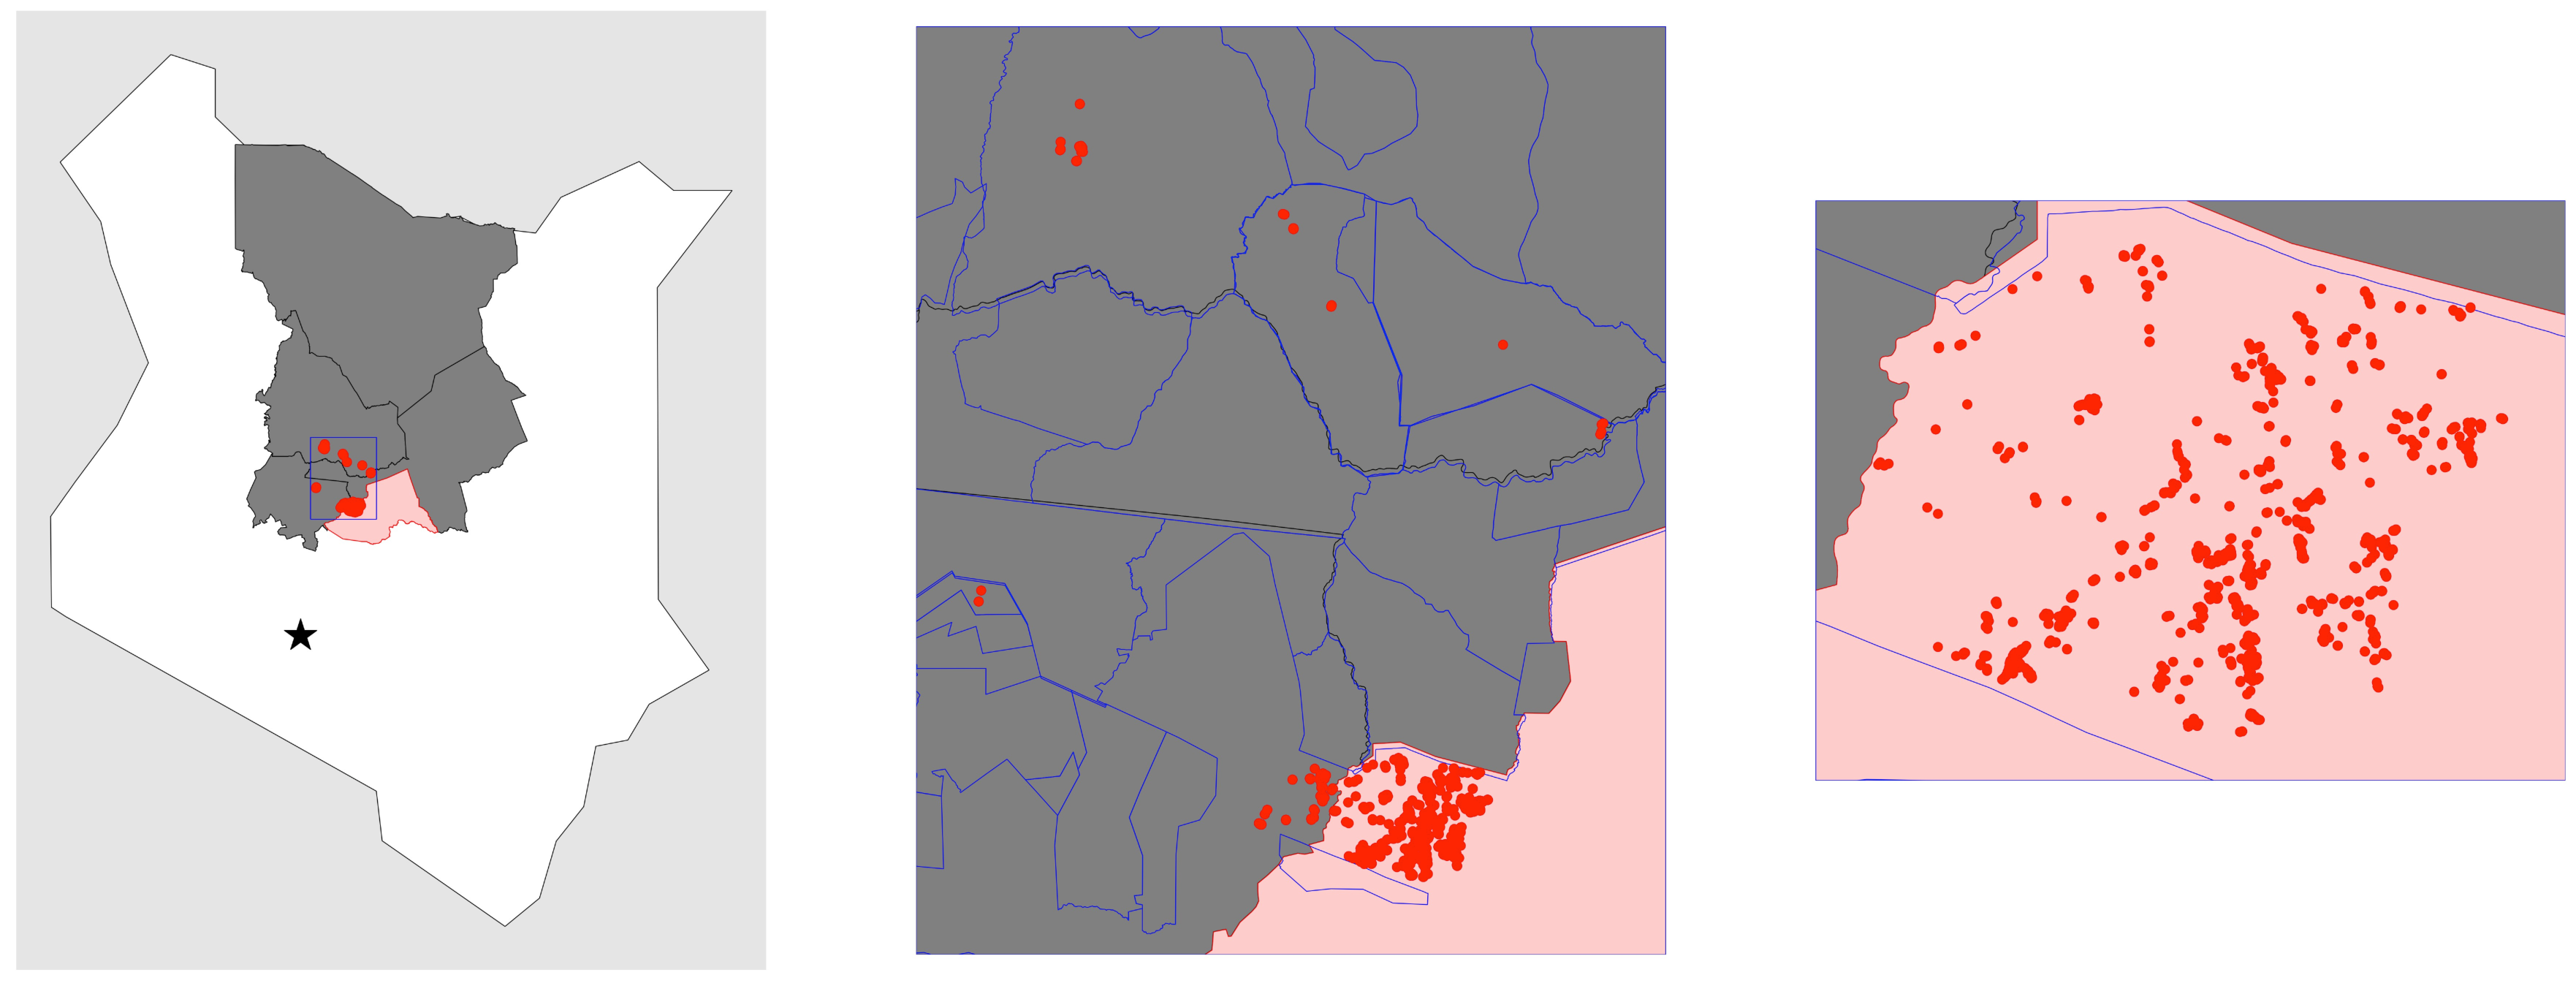
\includegraphics[width=0.90\linewidth]{resources/ca-map.pdf}
    \end{center}
    \caption{The map of image GPS locations in the GZCD dataset.  Meru County, Kenya (in red) is located north of the capitol (star) and is at the base of Mt. Kenya.  The dataset is comprised of 5,464 images, taken mostly over 4 days (2 days in 2016 and 2 days in 2018), by 13 photographers.  Includes all images by photographers that took images in Meru County, even if they were not taken in that county.}
    \label{fig:ca-map}
\end{figure*}

The dataset is highly curated; bounding boxes (annotations) and labels (species, viewpoint, and quality) were manually set for all animals to ensure accuracy and consistency.
The annotations in the dataset cover 23 unique object classes, ranging from ``gazelle'' to ``car'' to ``bird'' to two different species of zebra.  In total, 13,823 annotations were created, of which 9,205 were of Gr\'evy's zebra.  On average, 2.5 annotations were created per image, with one image contributing 44 annotations.  The photographers correctly followed the instructions to emphasize taking images of the intended sides of the animals (back-right, right, and front-right); human reviewers found a total of 7,372 annotations showing some degree of the right side.  Of these, blurry and otherwise poor images were filtered out using a human-labeled quality decision, keeping 4,119 candidate ``quality baseline'' annotations for ID review.  Figure~\ref{fig:ca-bad-examples} shows example annotations which are not useful for visual ID.  Furthermore, relatively poor-quality annotations were also needed to demonstrate that the filtering supplied by Census Annotations (described in Chapter~\ref{chapter:ca}) worked to improve matching.  The CA classifier for Gr\'evy's zebra was run with an exceptionally low threshold of 0.001 (compared to the recommended value of 0.31) to search for ``bad'' annotations but still filtered out abject ``junk'' annotations that showed nothing worthwhile.  An additional set of 1,162 low-quality annotations were added for the purpose of evaluating CA, and a resulting collection of 5,281 annotations was sent ID for curation.

\begin{figure}[!t]
    \begin{center}
        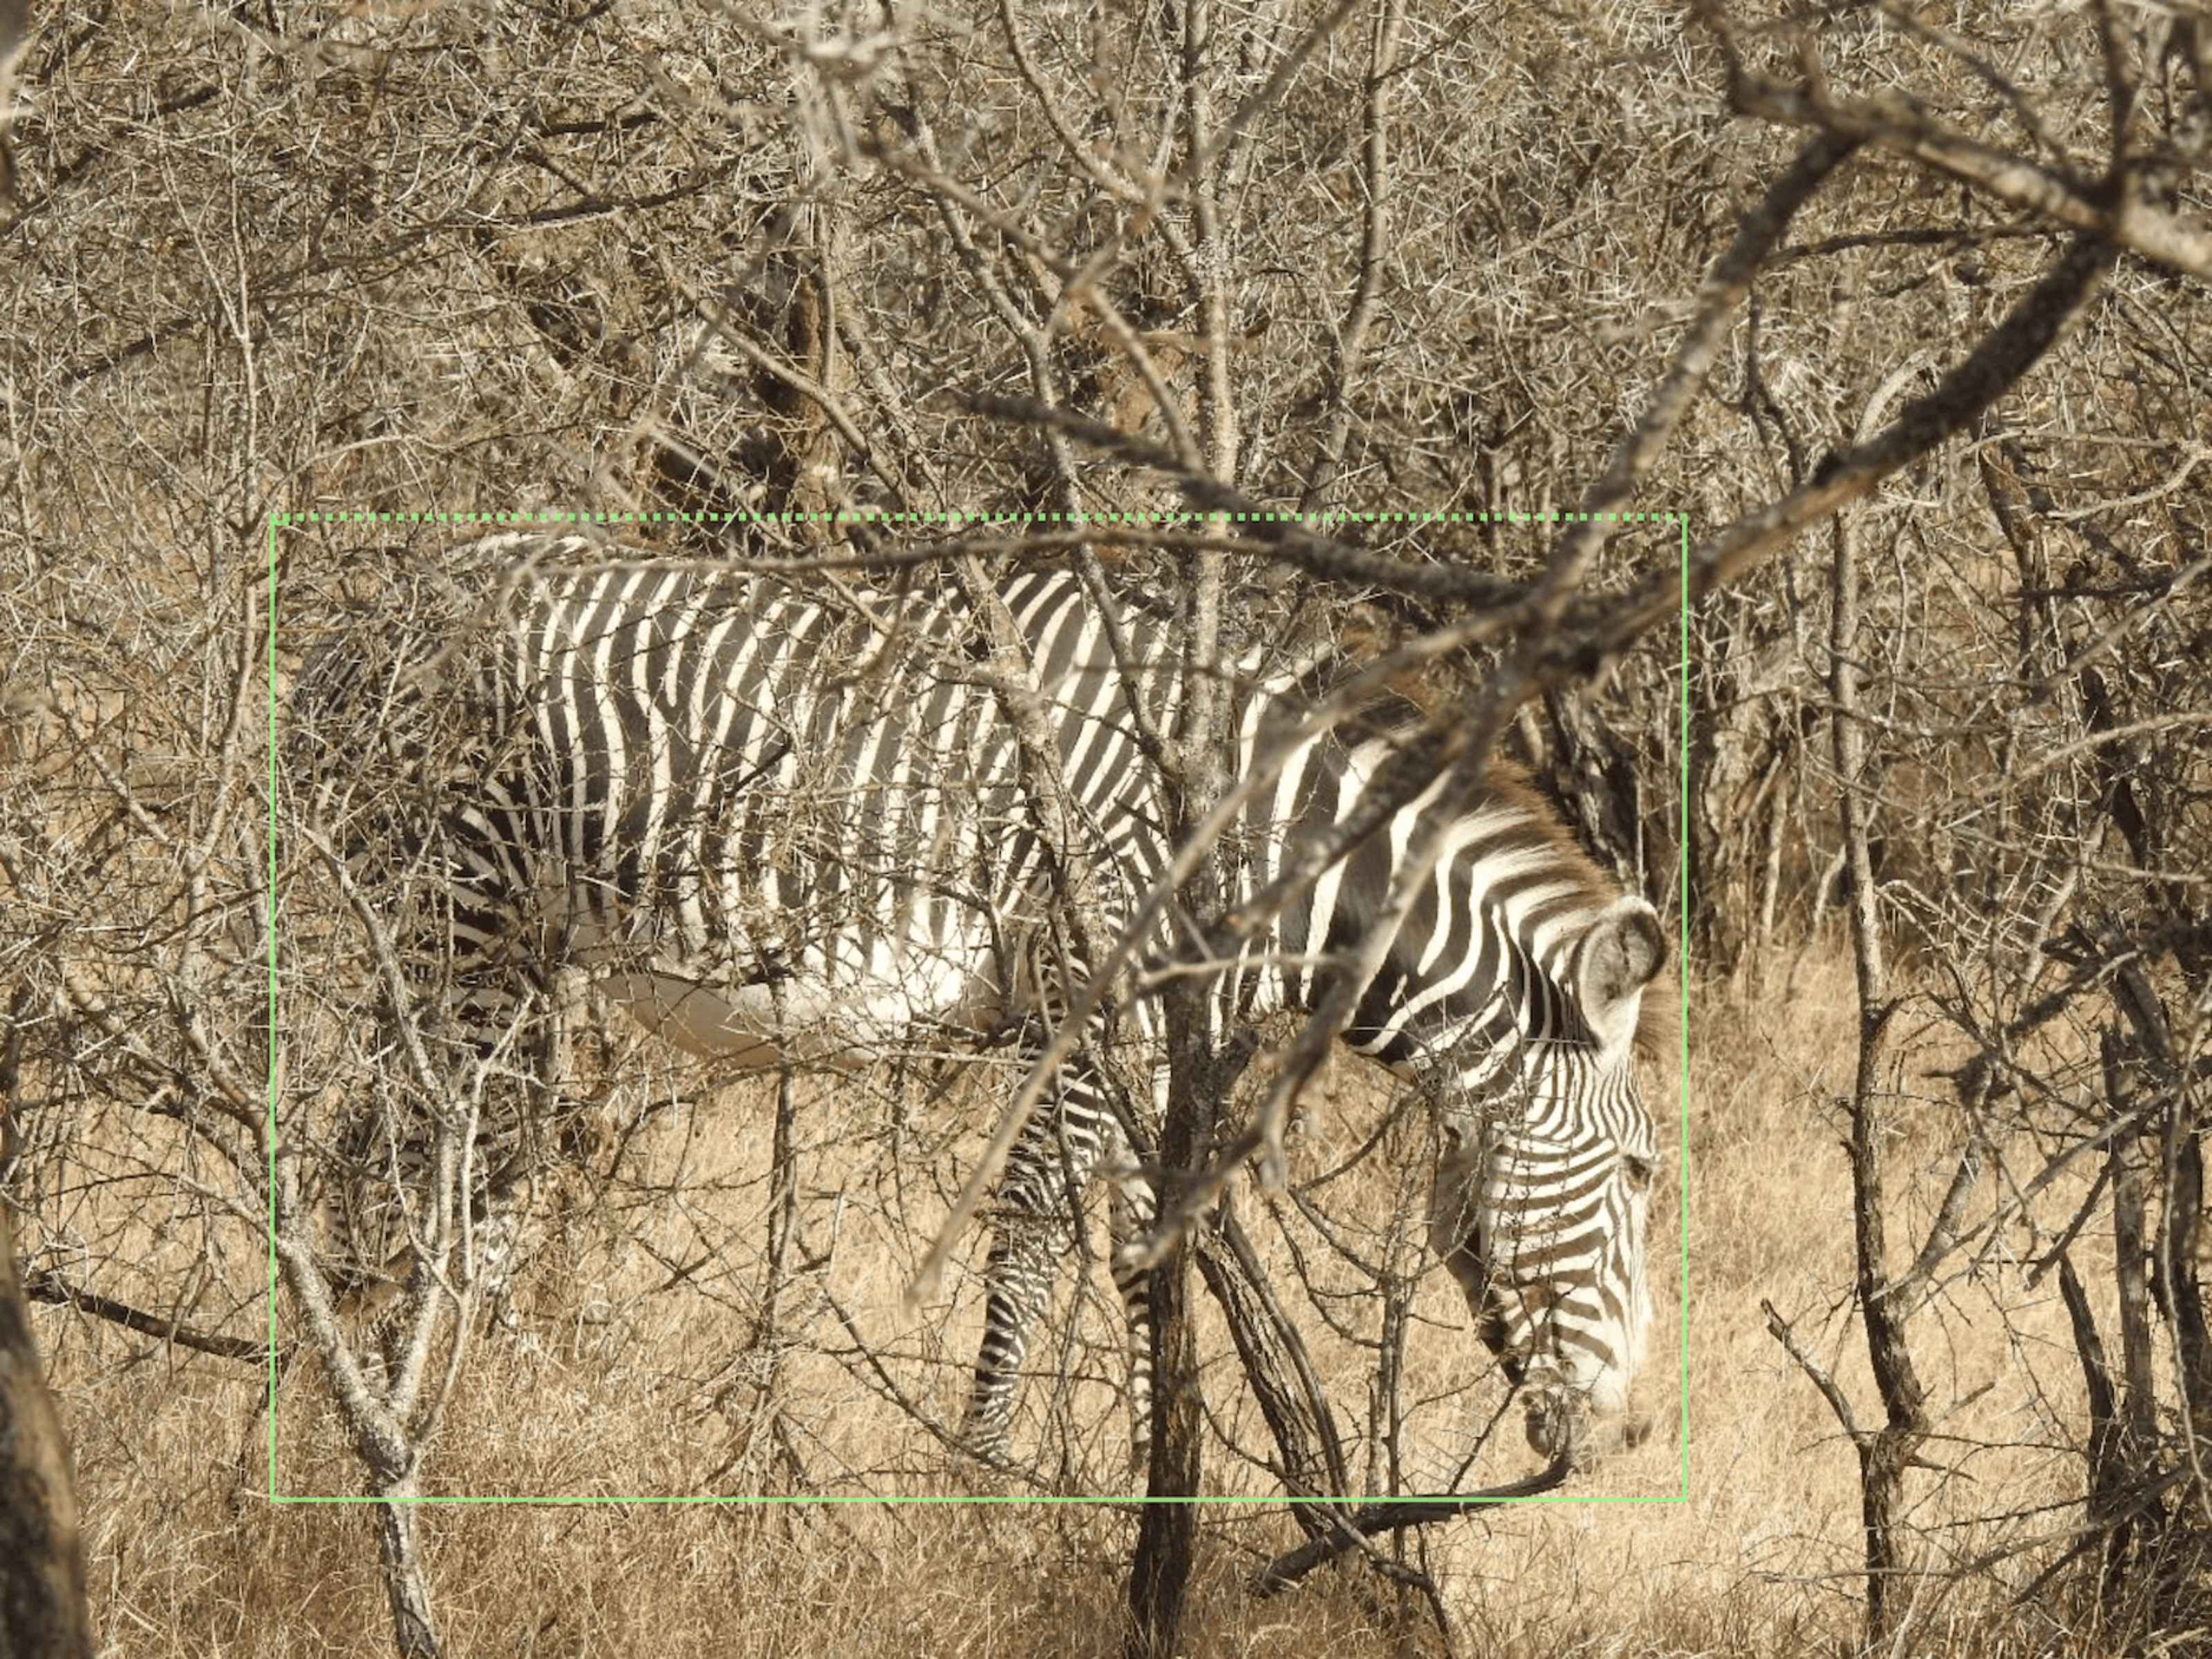
\includegraphics[width=0.31\linewidth]{resources/bad-occlusion1.pdf}
        \hspace{1mm}
        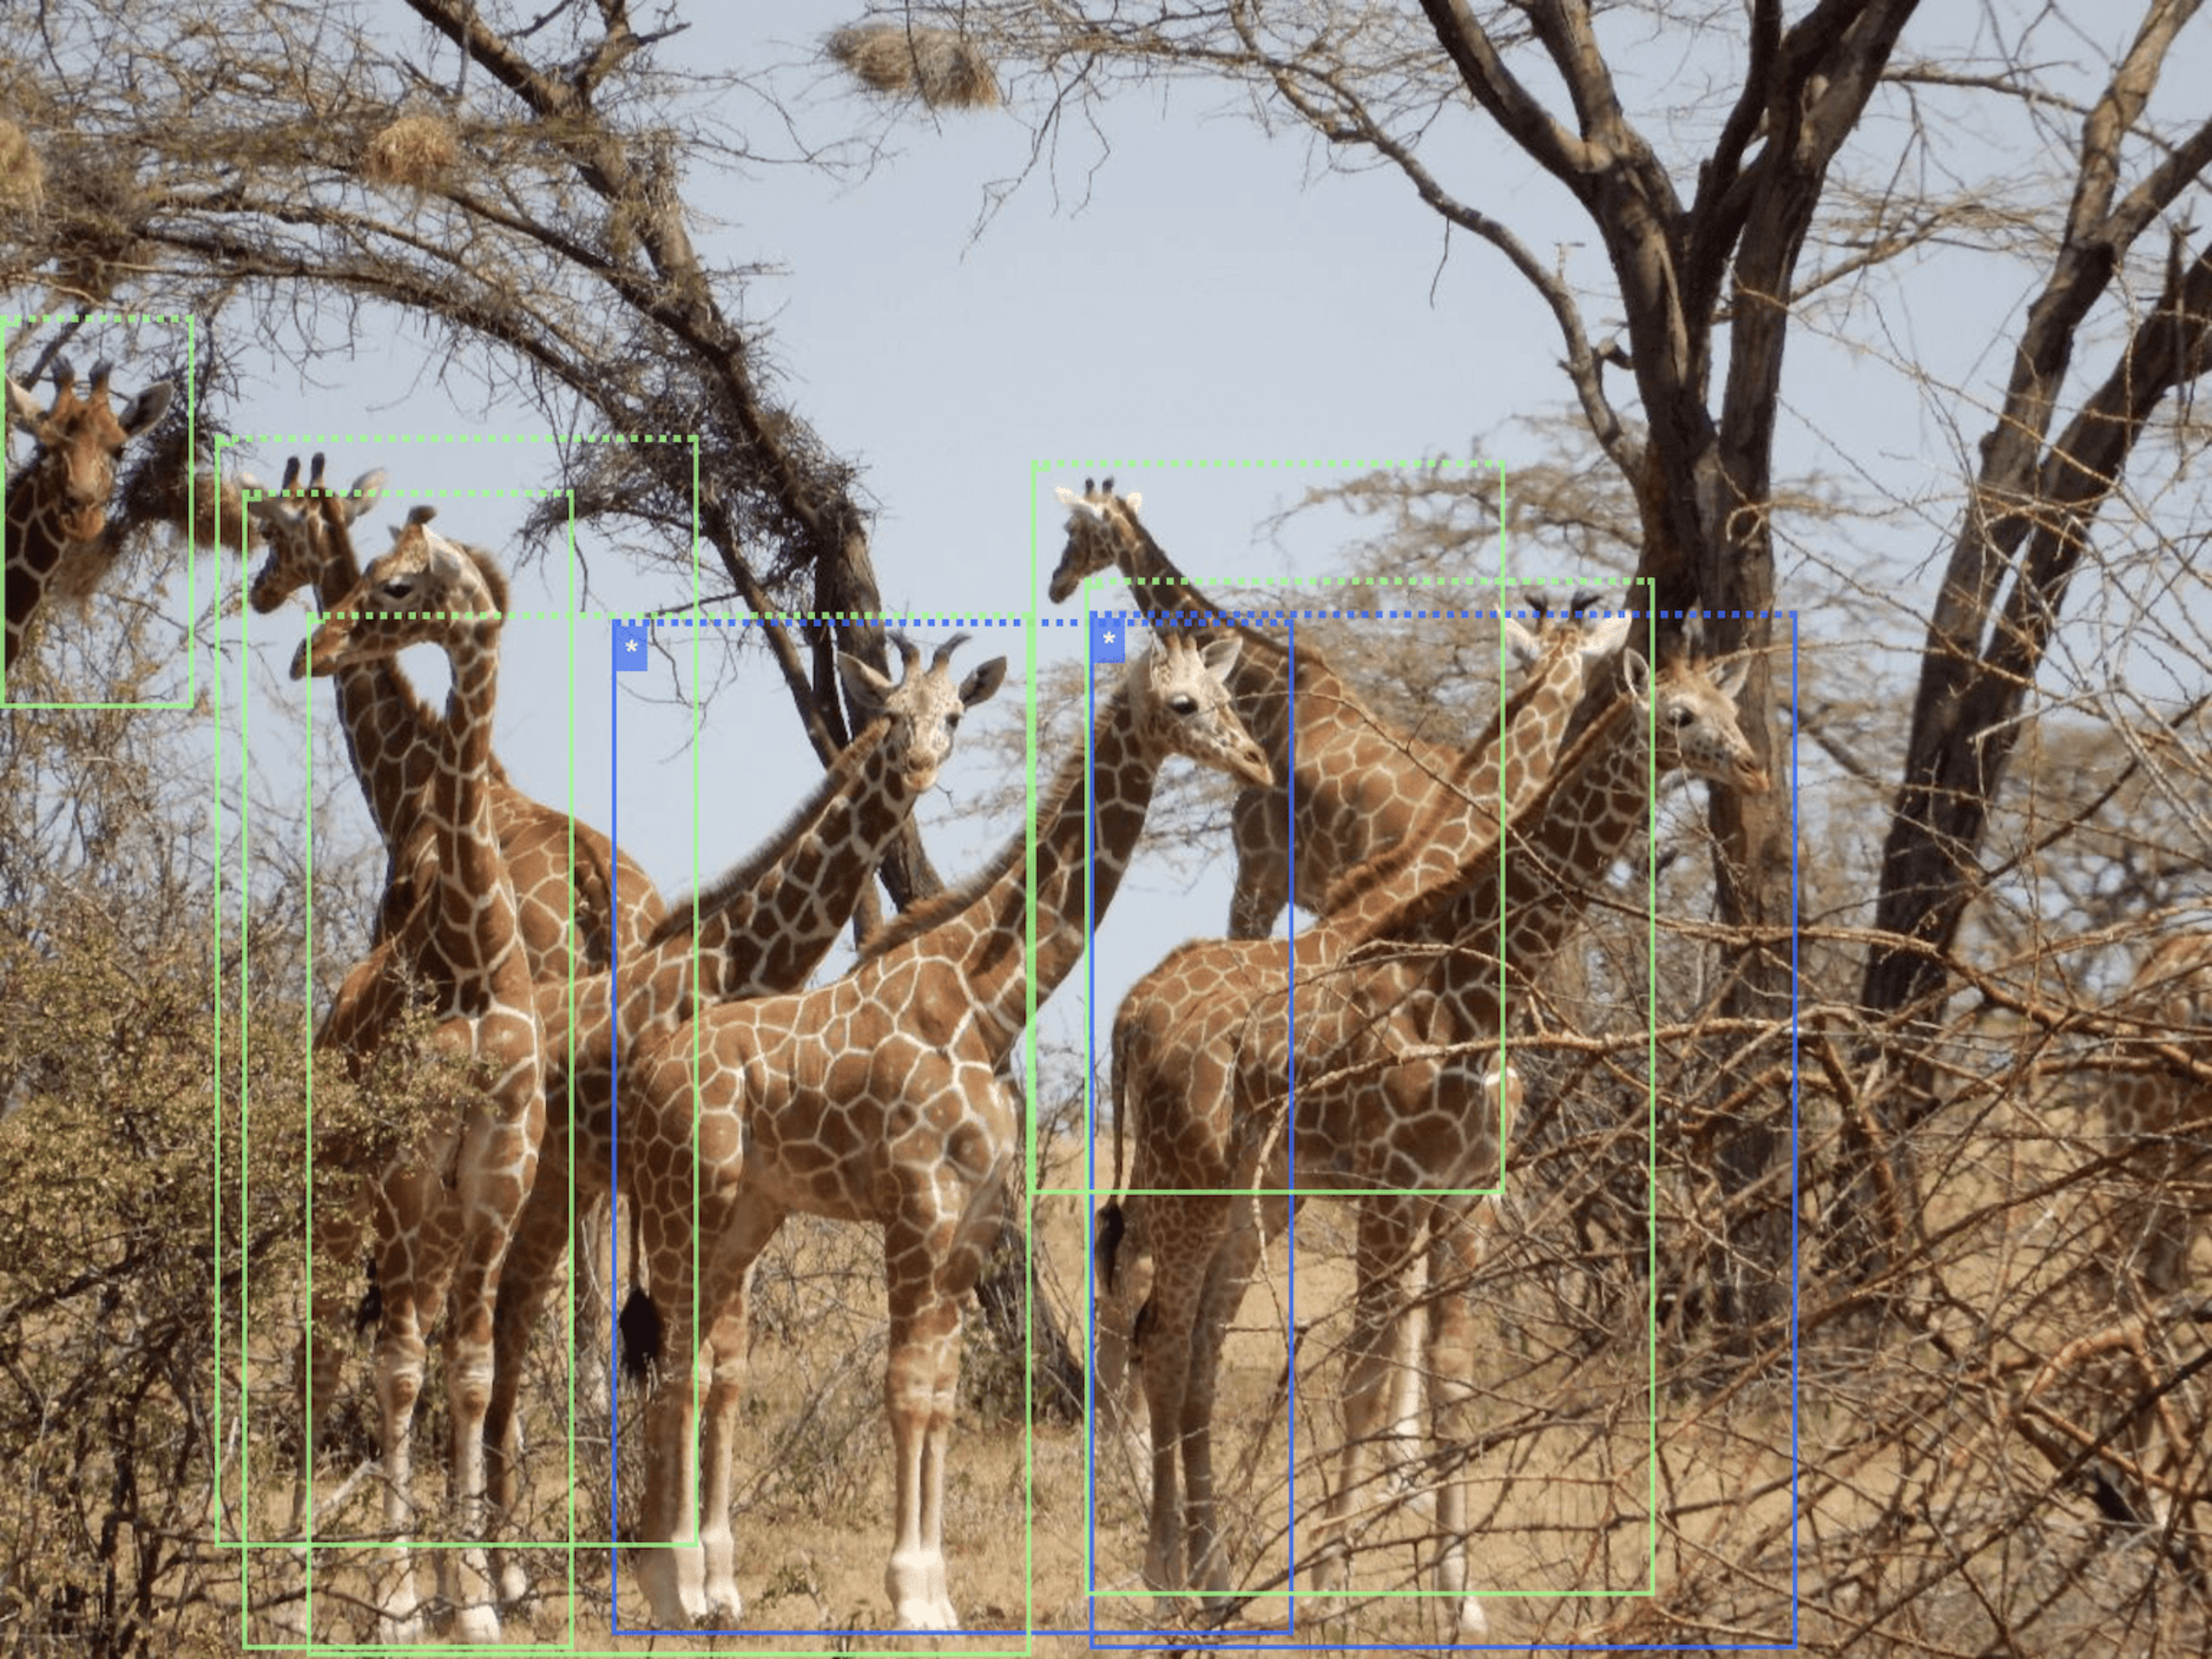
\includegraphics[width=0.31\linewidth]{resources/bad-overlap1.pdf}
        \hspace{1mm}
        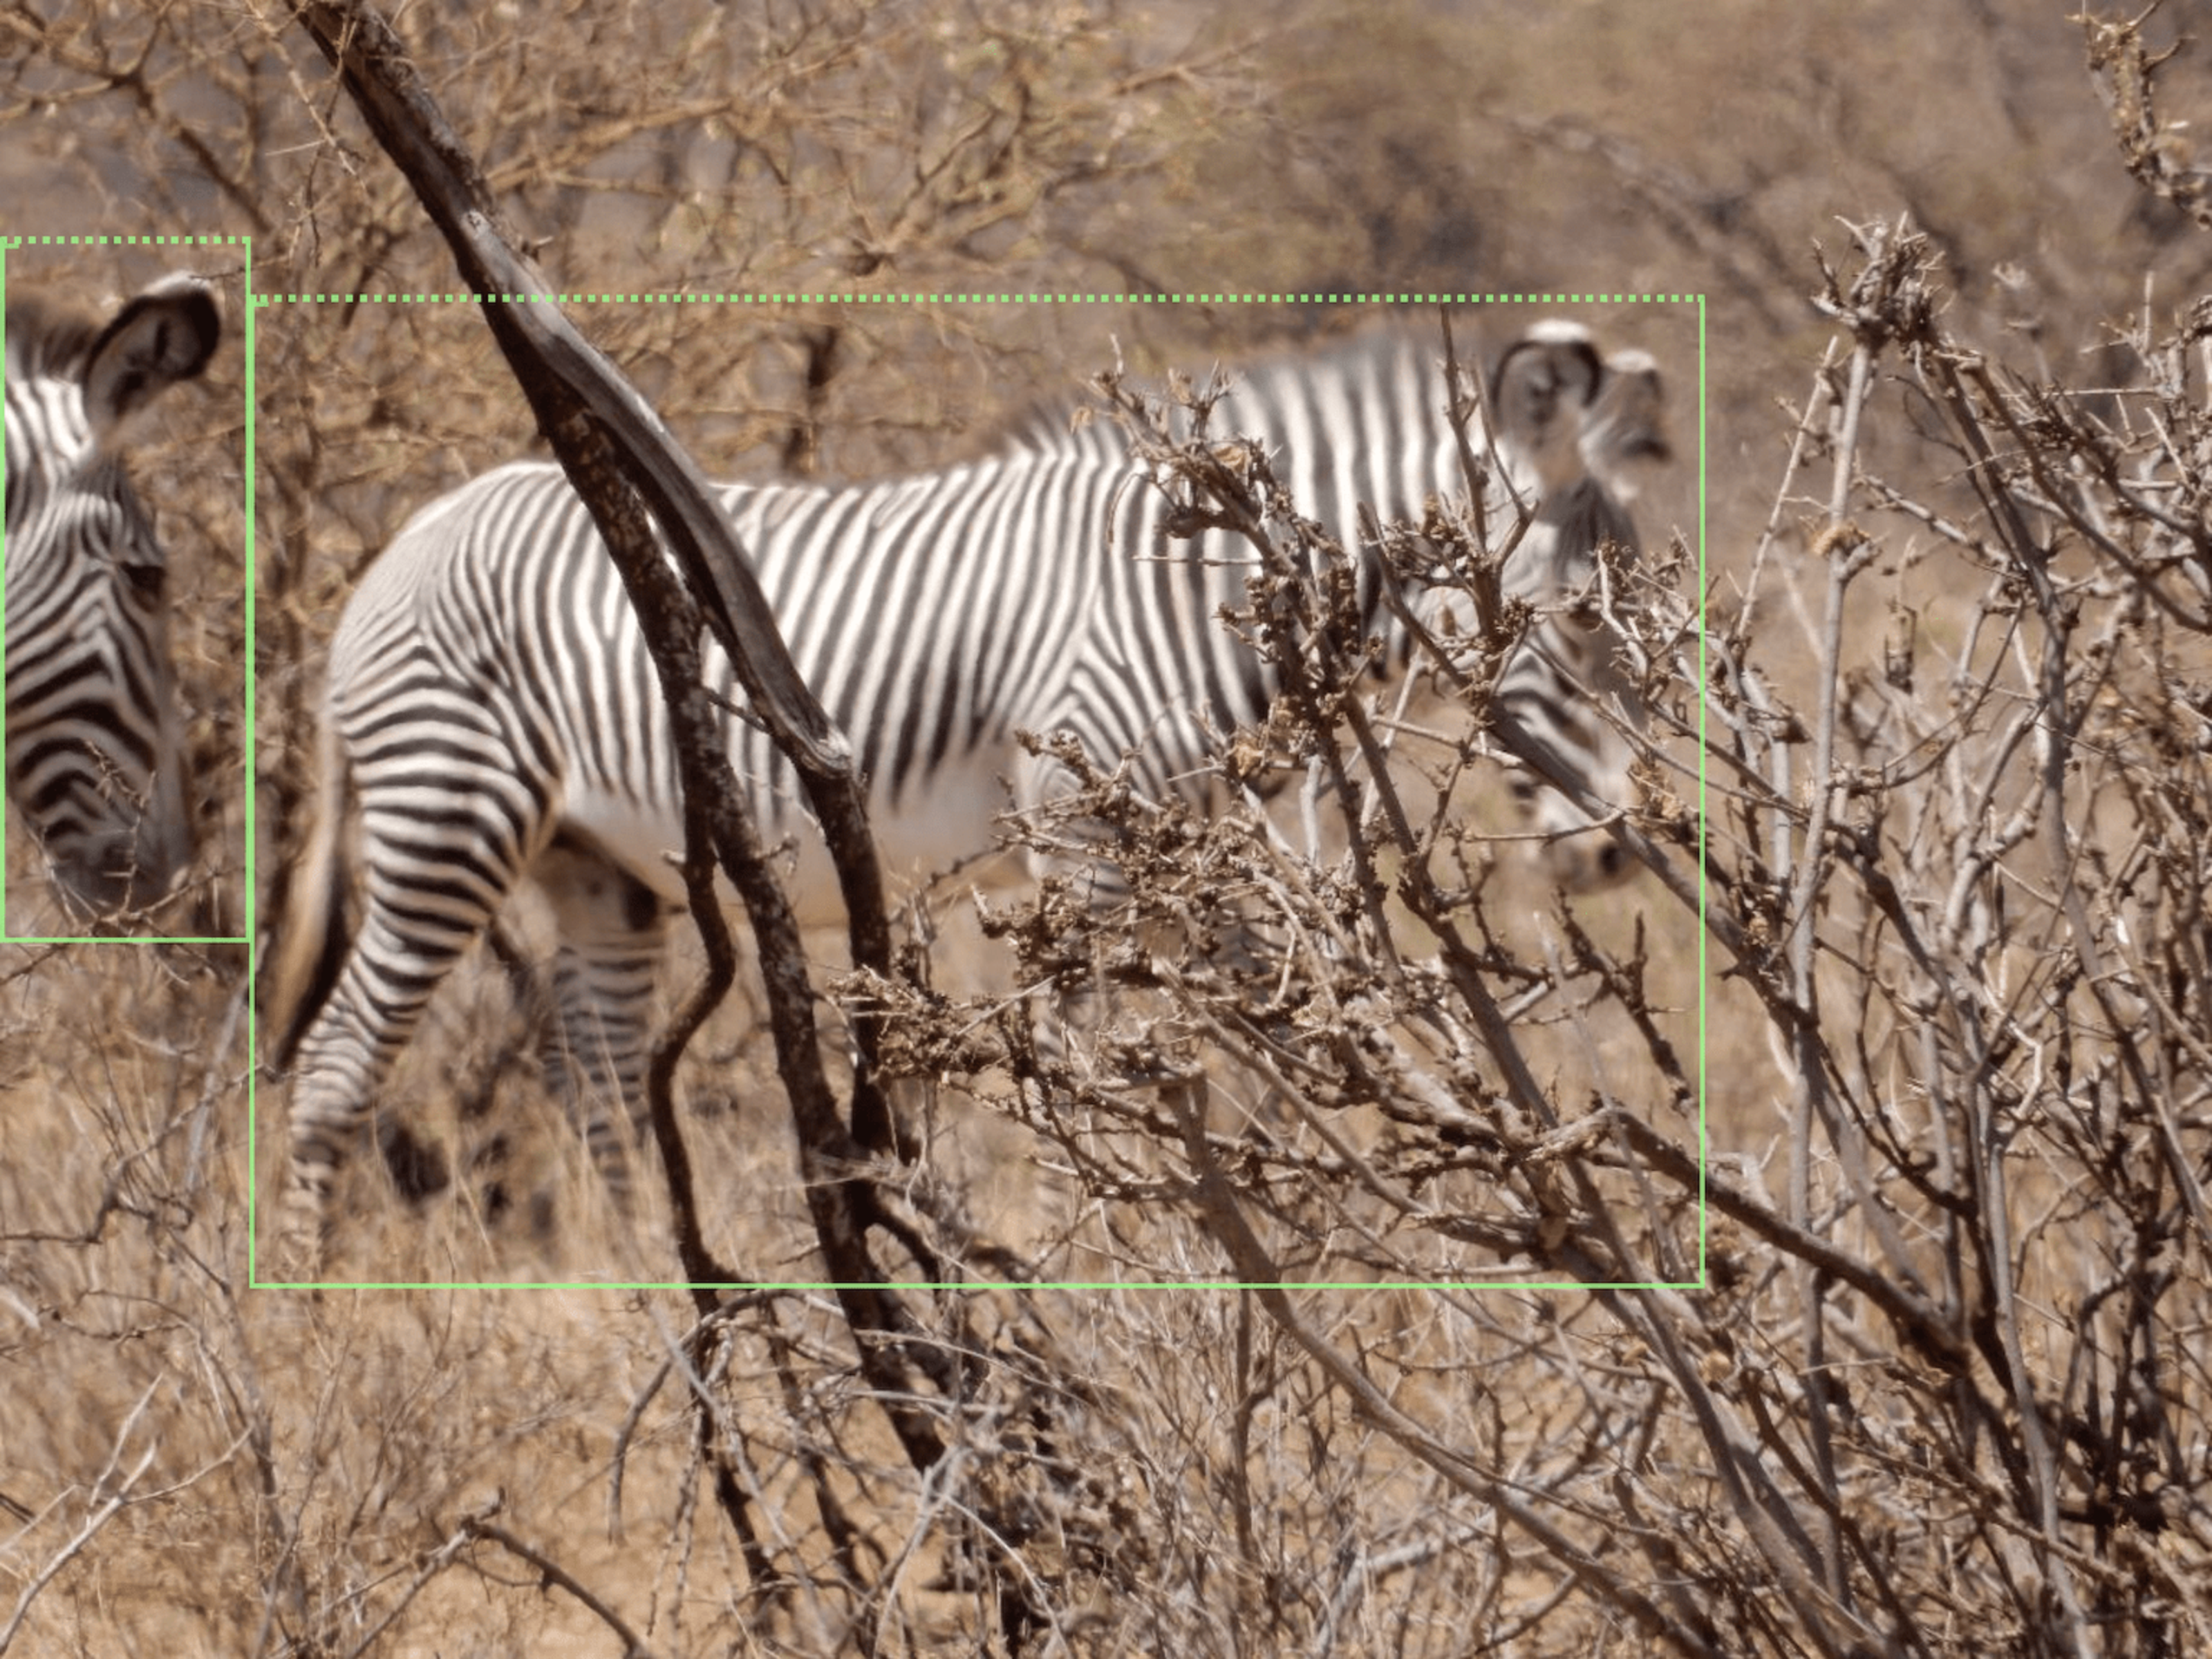
\includegraphics[width=0.31\linewidth]{resources/bad-quality1.pdf} \\
        \vspace{3mm}
        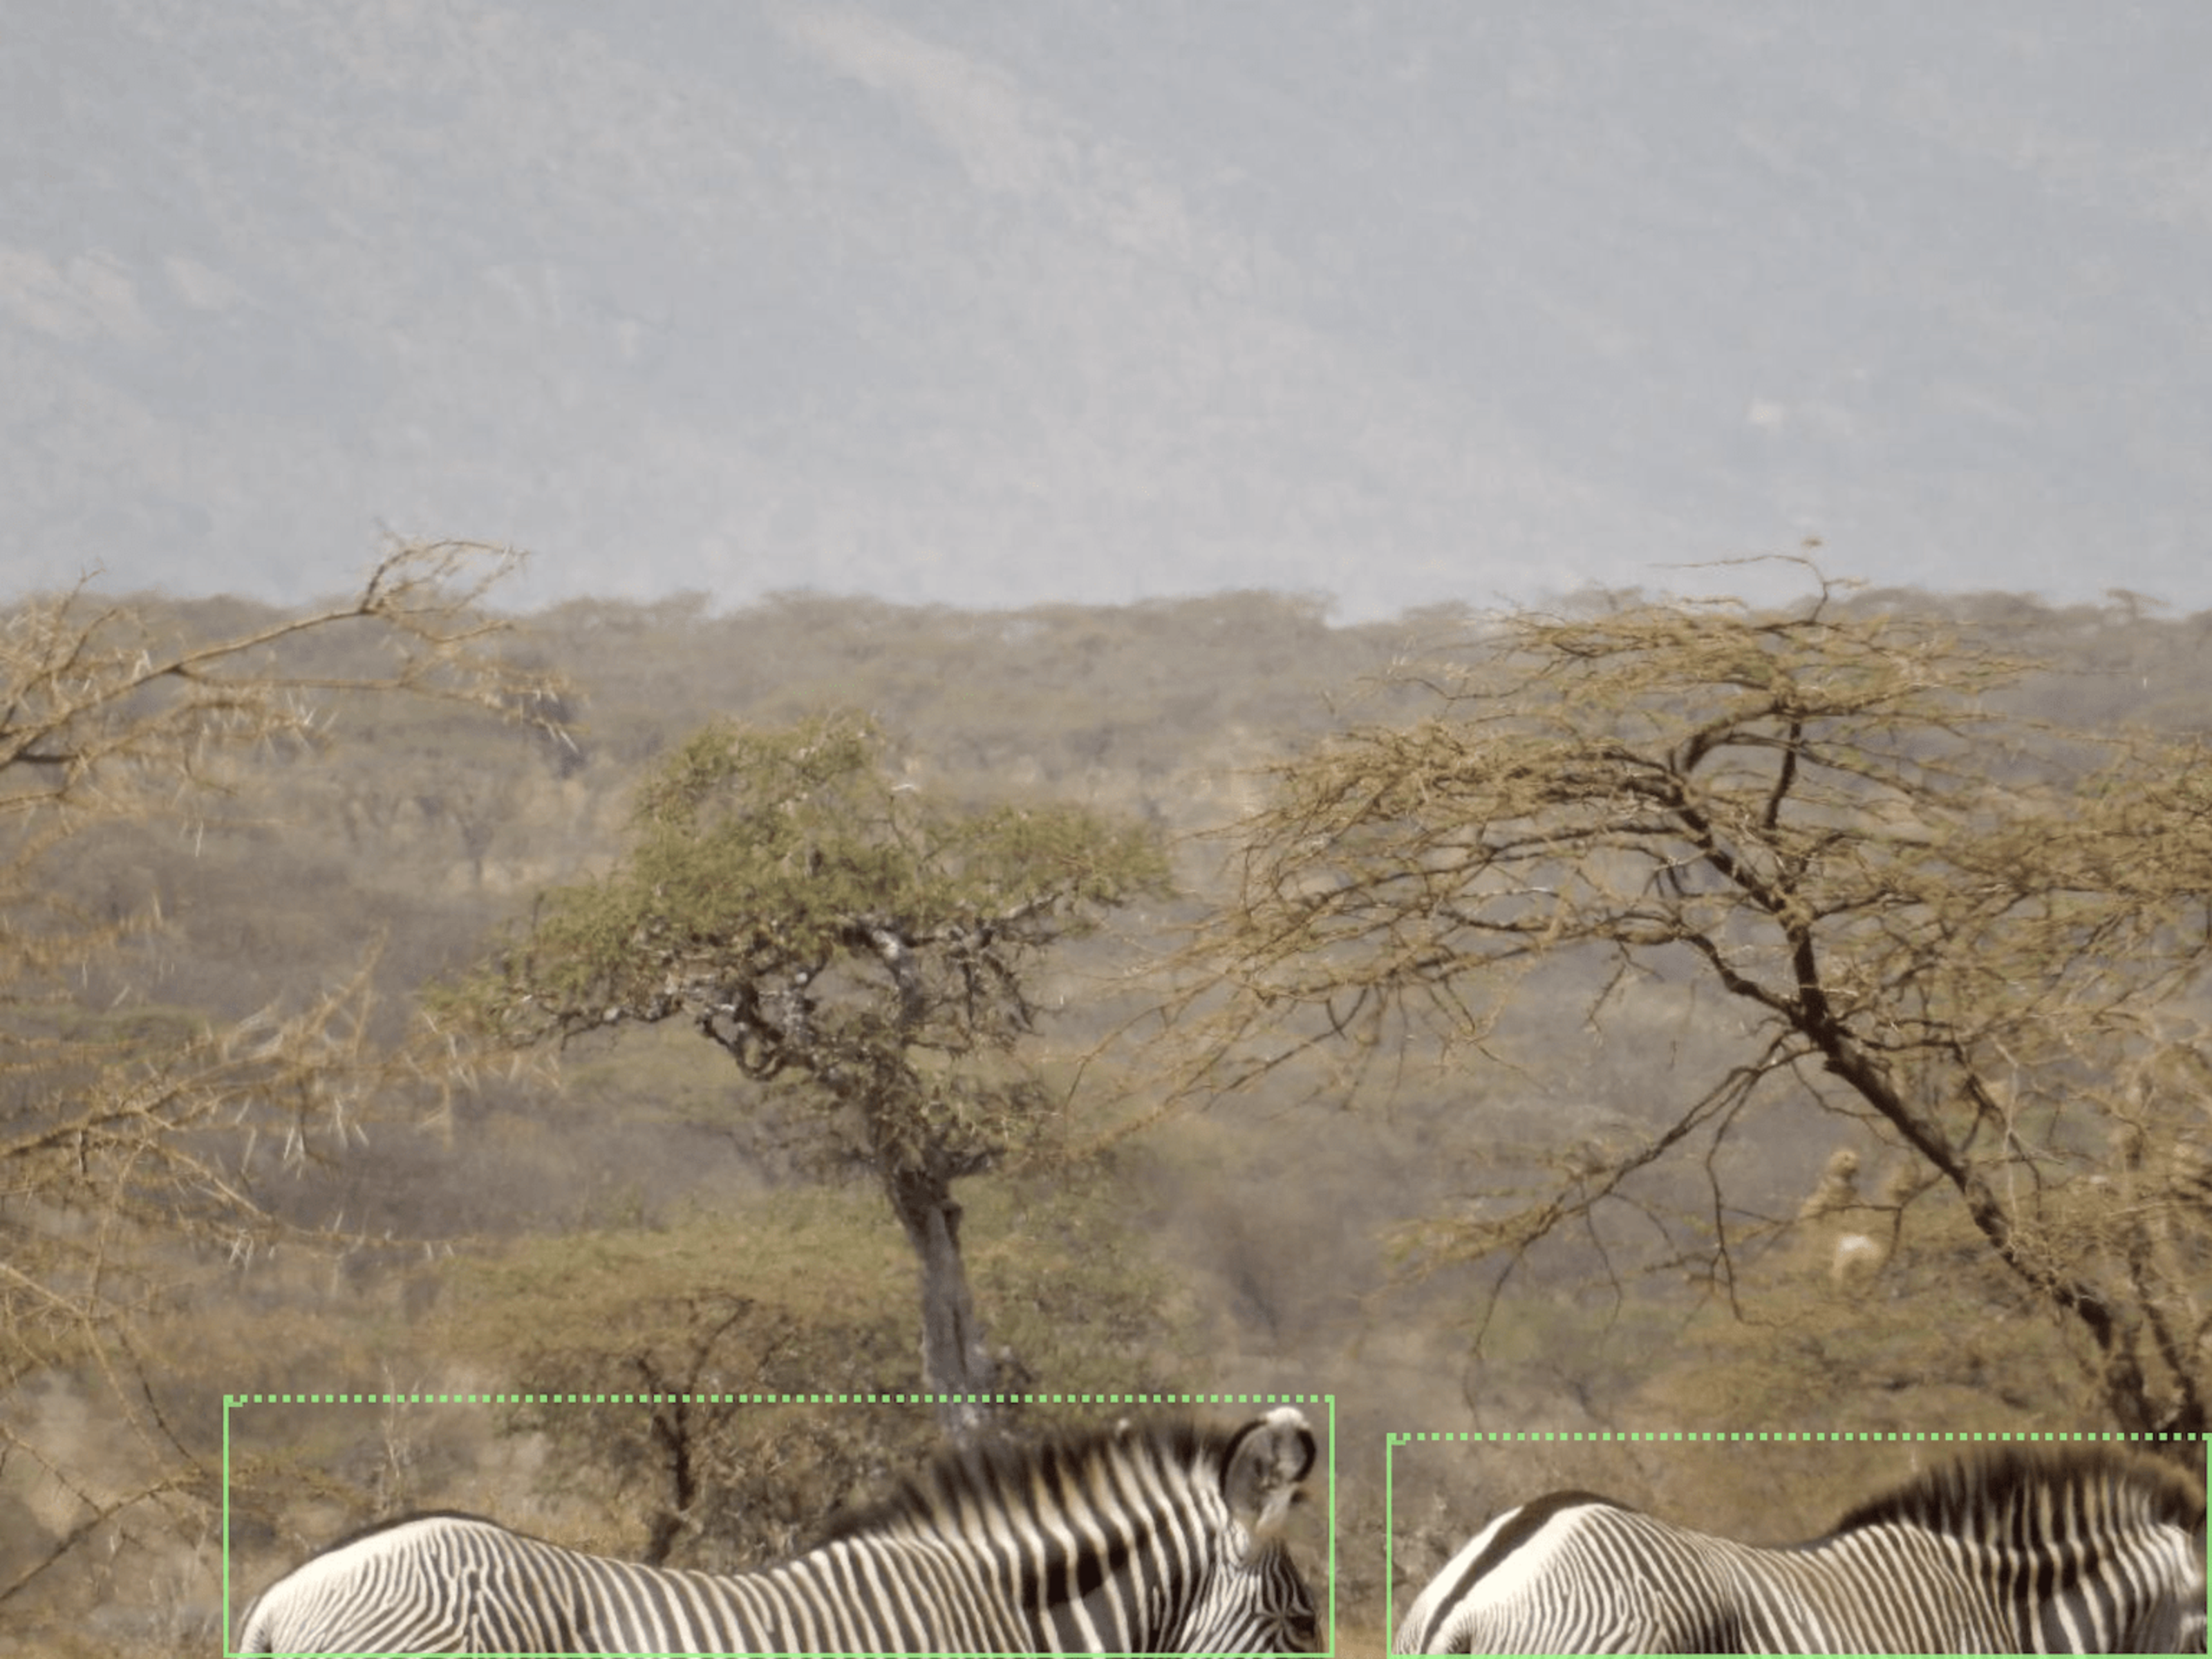
\includegraphics[width=0.31\linewidth]{resources/bad-truncation1.pdf}
        \hspace{1mm}
        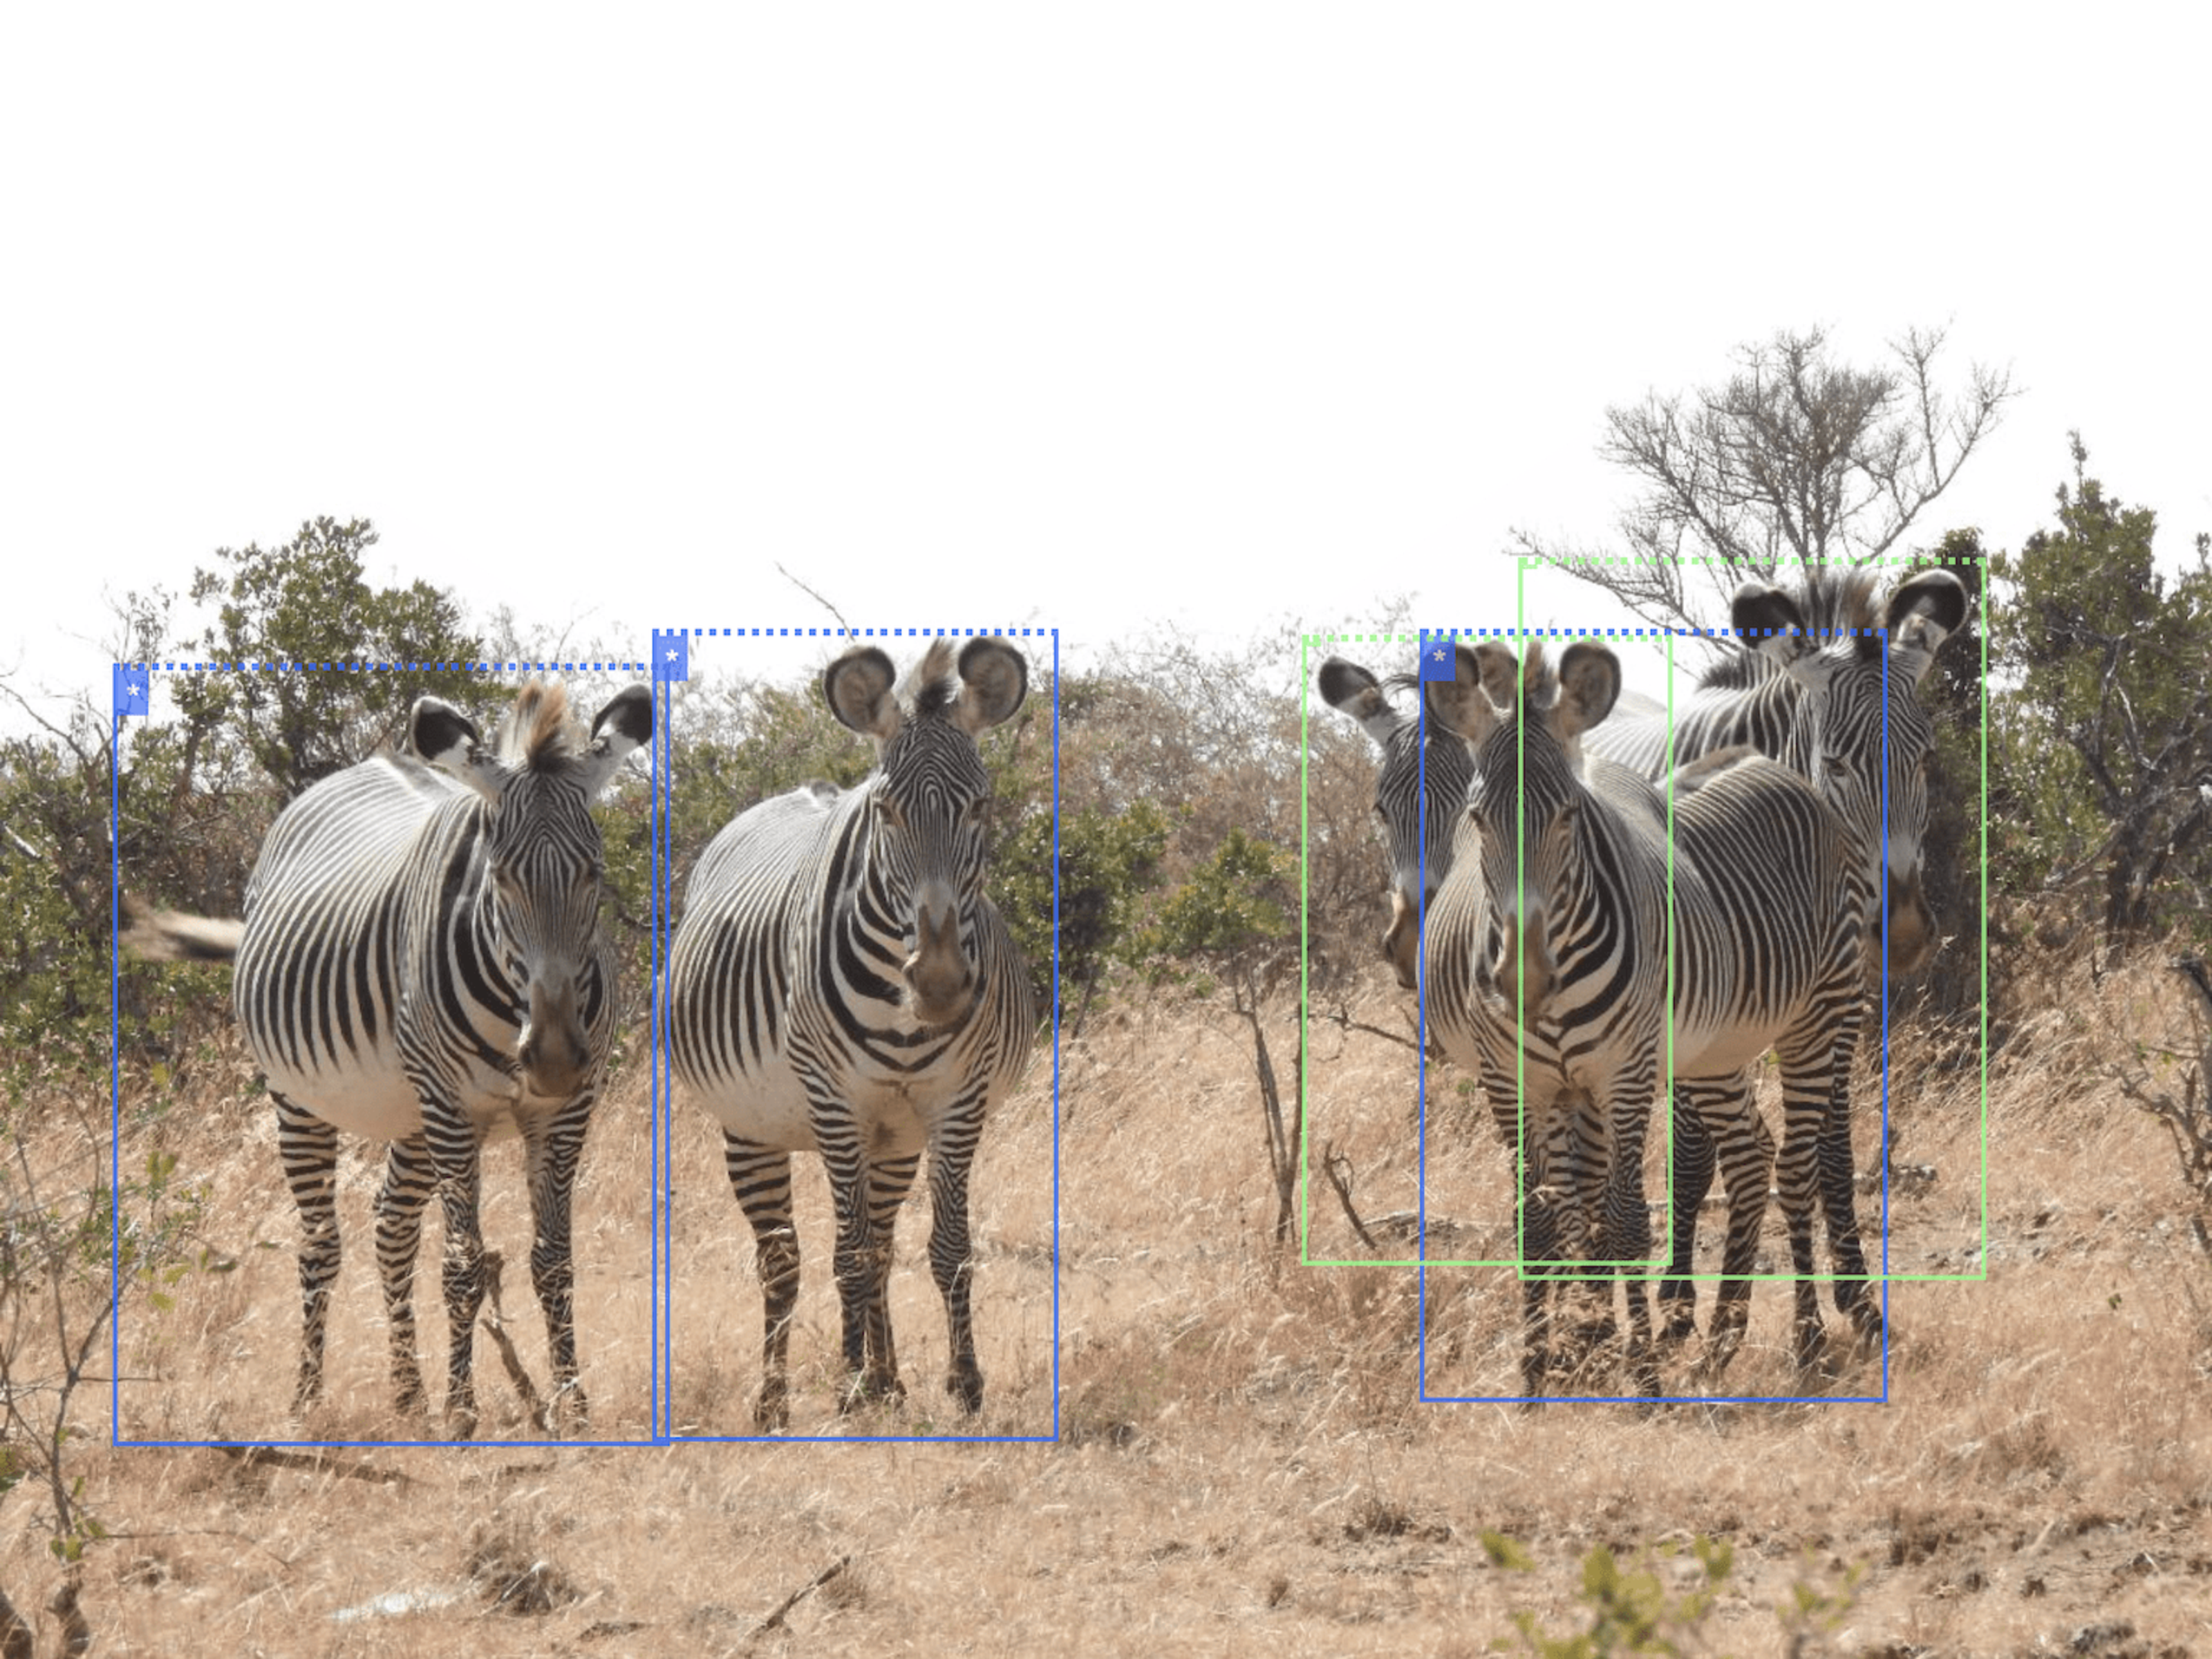
\includegraphics[width=0.31\linewidth]{resources/bad-viewpoint1.pdf}
        \hspace{1mm}
        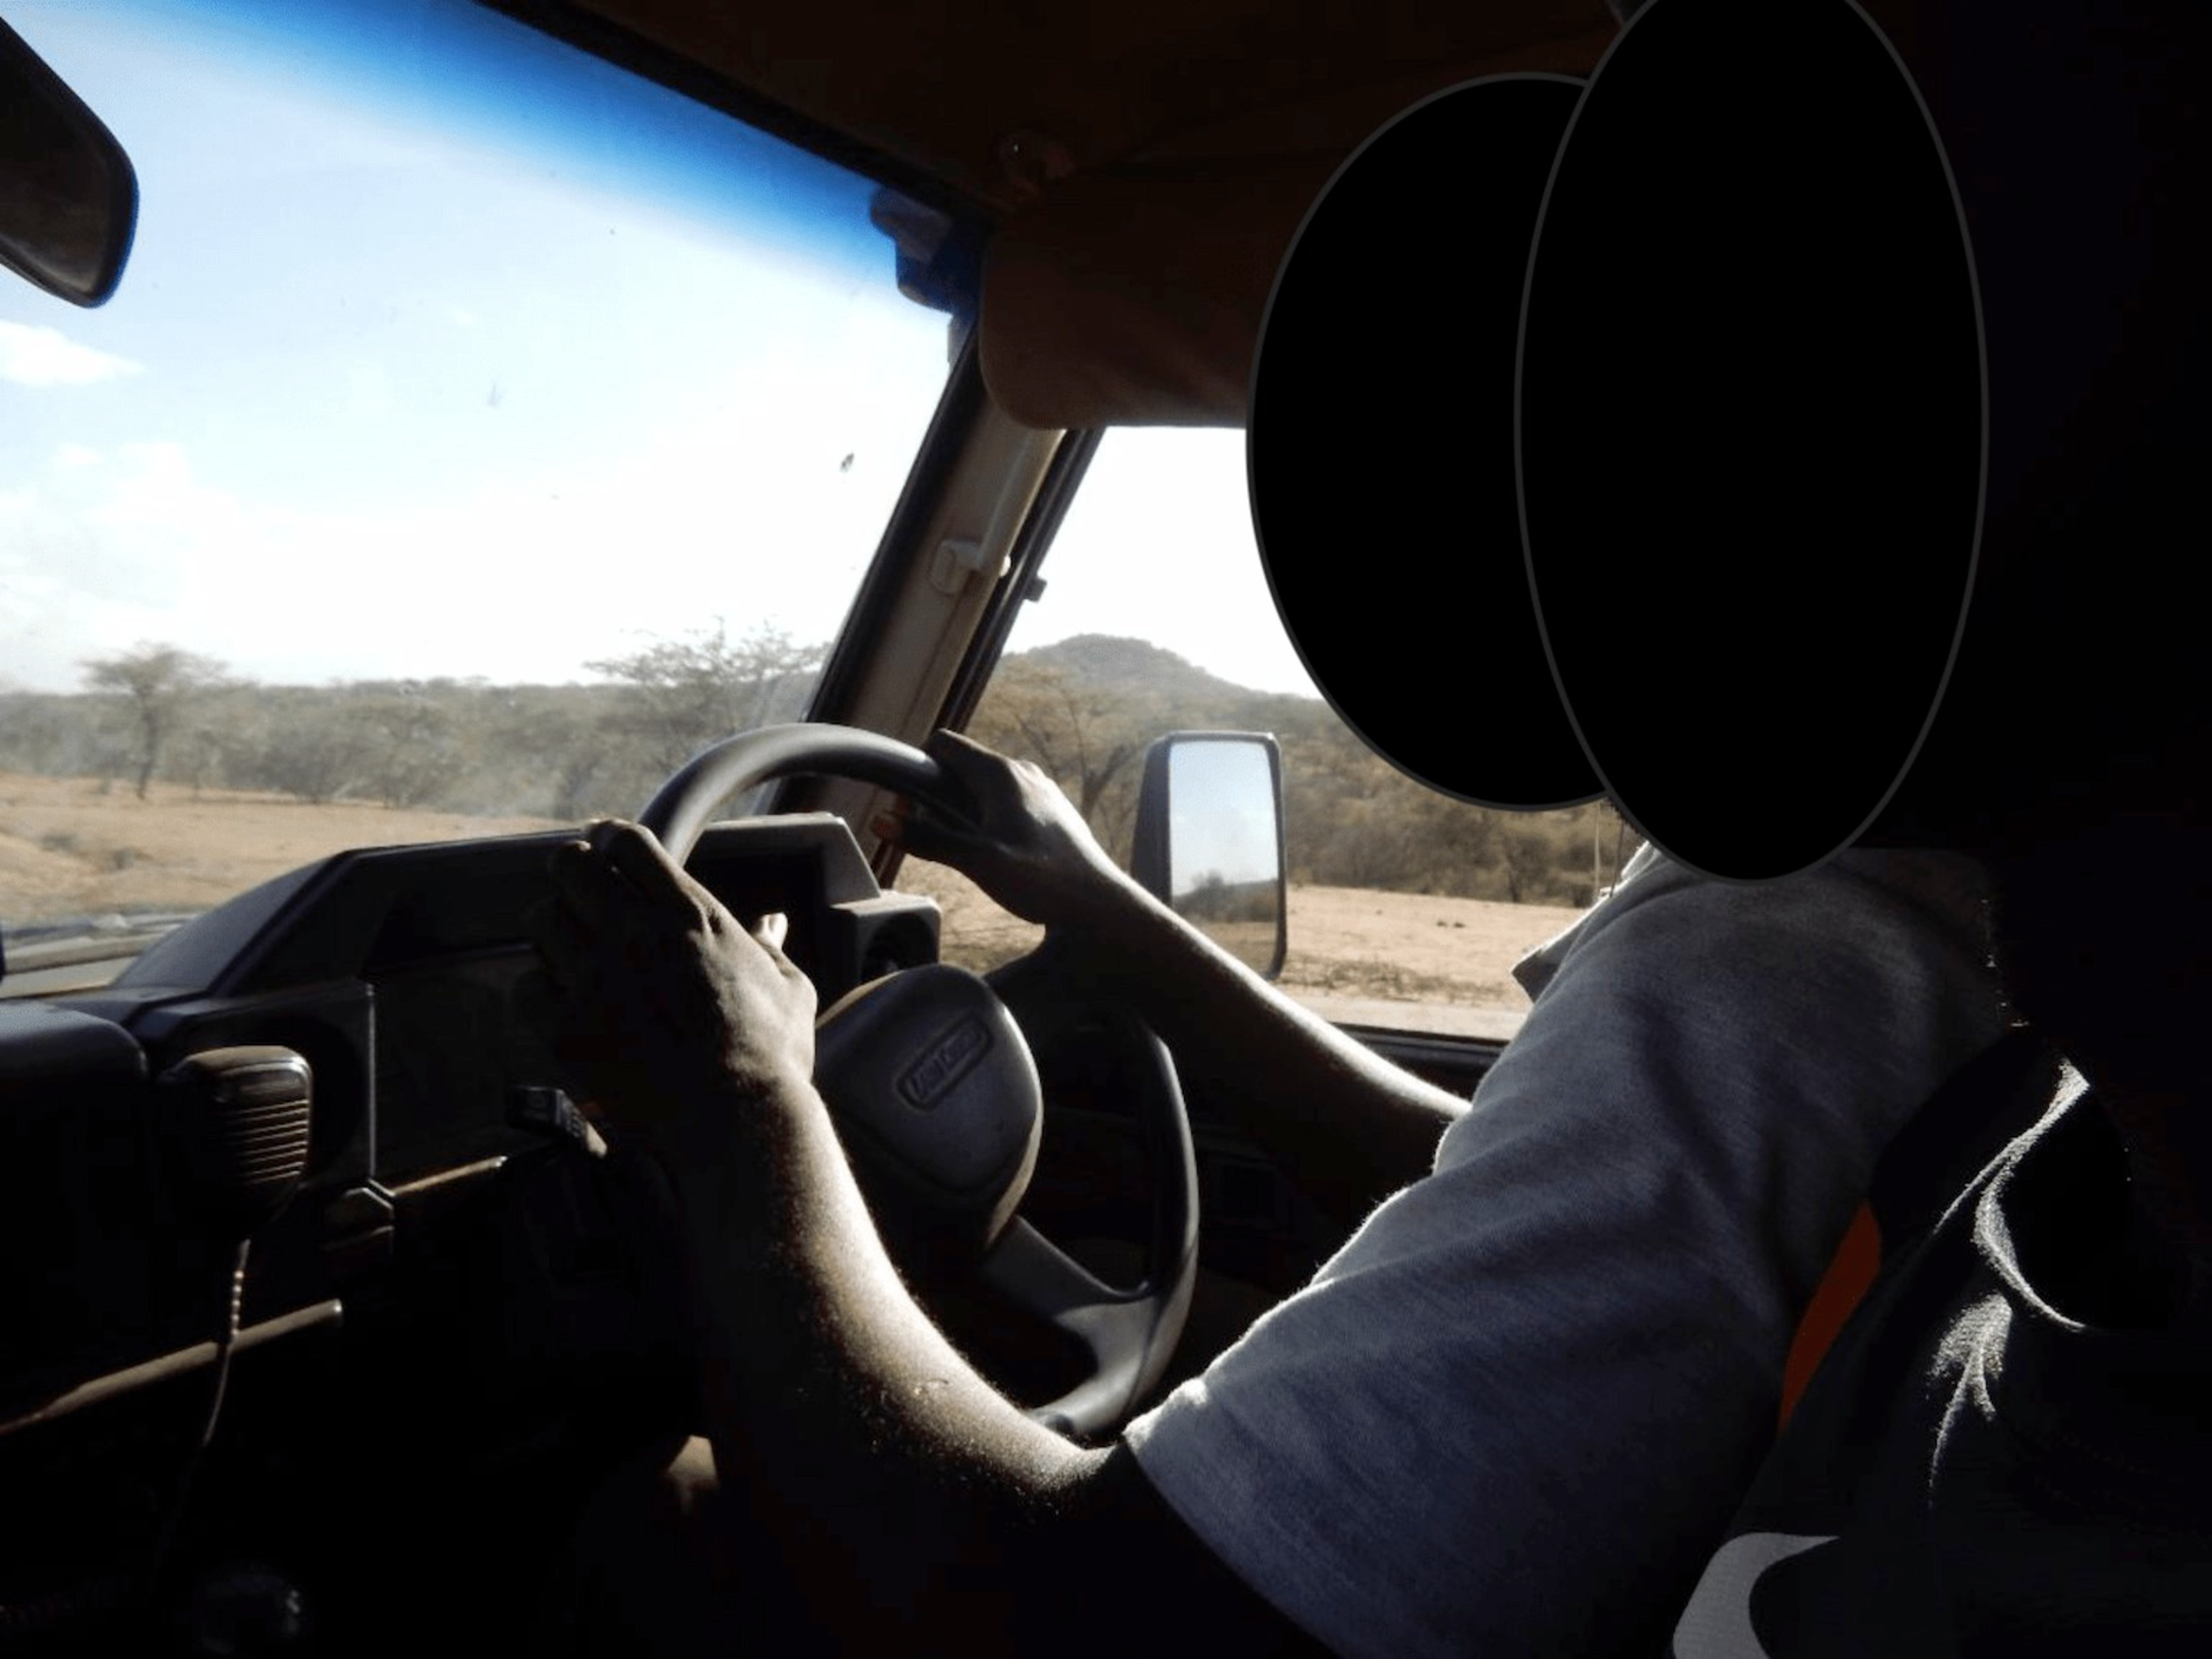
\includegraphics[width=0.31\linewidth]{resources/bad-context1.pdf}
    \end{center}
    \caption{Example annotations from GGR-18 that are poor candidates for identification.  These images are fairly typical (i.e. not extreme outliers) and demonstrate the various types of problems encountered by data collection (from top left to bottom right): (top row) occlusion, high amounts of overlap, quality (focus), and (bottom row) truncation, viewpoint/pose, and context.}
    \label{fig:ca-bad-examples}
\end{figure}

The state-of-the-art visual ranking algorithm HotSpotter~\cite{crall_hotspotter_2013} was used to find different annotations of the same animal.  The annotations were visually matched by creating a searchable database of SIFT features and generated results in a ranked list of potential matches. The graph of annotations was fully curated using this ranked list of matches and the Graph ID algorithm~\cite{crall_identifying_2017}.  The algorithm uses a series of phases that switches back and forth between adding positive decisions from ranking and ensuring that those decisions are consistent with the state of the graph as an automated classifier and human reviewers make decisions.  The algorithm has five distinct phases and begins with an initial recovery condition (phase 0) to ensure that the current graph has no inconsistencies.  An inconsistency is created when a chain of nodes connected by positive decisions also has negative decisions between two of its members (and vise-versa).  Once all inconsistencies are manually resolved, phase 1 continues by reviewing a list of match decisions recommended by a ranking algorithm.  Each pair was given to VAMP~\cite{crall_identifying_2017} using a pre-trained verification algorithm configured for Gr\'evy's zebra and was either automatically decided using a set threshold or was subsequently given to a human to make a manual decision.  This process continues until all of the decisions have been considered, and all inconsistencies are resolved.  After the initial ranking, pockets of nodes within the graph form positive connected components (PCC).  Phase 2 reinforces all of the PCCs in the graph by ensuring that each node has a set (two, by default) number of redundant positive decisions with another member of the connected component, searching for possible splits.  A negative redundancy check is performed in Phase 3 between all of the matched PCCs to ensure sufficient checks for unresolved merges. Finally, the algorithm converges in Phase 4 when all (or a statistically significant number) of the PCCs satisfy the positive and negative redundancy requirements, and its ID graph is free of inconsistencies.

In summary, 5,281 zebra annotations were clustered into 554 names, using 24,129 automated and 43,048 human pair decisions.  This work required thousands of hours of review by an external team of human reviewers.  Each annotation participated in 25.7 decisions on average ($\sigma$=34.3). Thus, the image data collected in Meru County during the two GGR events represented an ideal dataset for evaluation since it is self-contained, contains a sufficiently large population, and is highly curated.

\subsection{ID Curation \& Accuracy Verification}

Over 67,000 pairwise decisions were made using the Graph ID algorithm~\cite{crall_identifying_2017} to ensure that each cluster of annotations was internally consistent, representing a comprehensive (but not entirely exhaustive) review of the population graph.  The Graph ID required \textit{each} annotation within an animal ID (representing a single named zebra) to have at least two positive decisions with other annotations in the same cluster, whenever possible.  This redundancy requirement ensured that a given name did not incorrectly contain multiple animals by mistake, otherwise requiring a split and increasing the number of names.  We also configured the algorithm to require each animal ID to have at least two negative decisions between all other matched IDs.  This requirement ensured that a given cluster did not need to be combined with another.  Otherwise, the database would require a merge, and the number of names would decrease.  In total, each annotation, on average, participated in 5.5 positive and 20.0 negative decisions.  The effort required to create this dataset involved hundreds of hours of human labeling, months’ worth of review, and over \$10,000 in direct payments for external labor.

The ML-based automated decision classifier used for approximately 40\% of the decisions was not a perfect oracle.  The algorithm (VAMP~\cite{crall_identifying_2017}) was configured to allow positive and negative decisions if the predicted confidence was above a threshold, 0.7732 and 0.8605, respectively.  Based on cross-validation results, these thresholds were selected with validation data to allow an FPR $\leq 1\%$.  Since the Graph ID algorithm enforced redundancy and ensured consistency, there are likely to be few name errors resulting from using this automated classifier.  The chance of systematic errors is even less likely because each annotation participated in 16.3 ($\sigma$=28.6) human decisions on average.

The experimental LCA algorithm was then run on the final clusters produced by Graph ID to identify possible ground-truth errors and further validate the GZCD.  The PIE triplet-loss algorithm was also trained on the ground-truth IDs on Census Annotation Regions.  The verification of the ID database was performed in multiple stages of review, using the following combinations: Graph ID with HotSpotter as the ranker and VAMP as the verifier (legacy configuration), LCA with HotSpotter and VAMP, LCA with HotSpotter and PIE, LCA with PIE and VAMP, and LCA with PIE as the ranker and PIE (as well) as the verifier.  Each round of verification simulated the final state of the database using the ground-truth human decisions already in the database.  When the converged animal ID database was calculated, it was compared to the existing ground-truth database, and differences were examined by hand.  The first comparison identified 37 ID updates that performed 14 splits, 13 merges, and corrected 10 miscellaneous labeling errors.  The split cases were identified as challenging photobomb examples, which had animals seen together on multiple occasions and 1 mother/foal example (originally VAMP false positives).  A benefit of using this additional check is that some animal IDs were suggested to be split by removing only one annotation, which identified inappropriate (i.e., poor quality) annotations that needed to be discarded.  The merge issues found by the PIE ranking algorithm mainly were concerned with adding a singleton ID into a larger ID for the same animal (Graph ID retrieval errors).  It was apparent during a review that some errors were caused by poor quality annotations or had a very oblique angle (ground-truth labeling error).  Once all animal IDs were fixed in the database, no further corrections were identified from subsequent simulations and a manual review of their suggested changes.  In summary, the final GZCD database is found to be consistent by the following: two detection filtering configurations (baseline quality annotations and CAs), two separate ranking algorithms (a hand-engineered feature and learned embedding), two decision management algorithms (one that ensures positive/negative redundancy and another on cluster stability), two verification algorithms (random-forest classifier and a distance-based embedding), and over 43,000 human verification decisions of annotation pairs.

Any ID analysis of the number of annotations and names must also consider \textit{encounters}.  An \textit{encounter} is defined as an animal that is seen during a single \textit{occurrence}.  An occurrence is the collection of all images that are taken at the same location and time.  Another way of phrasing this: if a photographer took ten pictures of the same animal within one second, that would result in ten unique annotations but still only one encounter of that animal.  If ten photographers each took ten pictures of one animal during the same occurrence, that would result in 100 annotations but still only one encounter of that animal.  This analysis is intended to identify how many unique encounters an animal has because it represents a more accurate semantic understanding of how many times an animal is truly \textit{resighted}.  For a population estimate, the number of animals that were \textit{sighted} (or encountered) on days 1 and 2 of a given census can be calculated and compared to the number of animals that were encountered on \textit{both} days (resightings).

The number of occurrences was calculated using an agglomerate clustering of GPS coordinates and EXIF times provided by the GPS-enabled cameras.  We assumed a maximum speed of 2 m/s for a walking zebra and required that images be taken within 10 minutes.  The dataset offers 296 unique occurrences and 1,803 encounters of zebras.  The average occurrence has 25.1 named zebra annotations but only 8.6 encounters, indicating that each encounter contains around 2.9 annotations on average.  The amount of review redundancy for encounters is dramatic, with 51.2 total decisions on average.  In summary, the dataset contains 554 uniquely named zebras, with 9.5 ($\sigma$=8.4) annotations and 3.3 ($\sigma$=2.2) encounters per name on average.  There are 95 names that contain only one annotation (and trivially only one encounter) and are referred to as \textit{singletons} against the remaining 459 \textit{multitons}.  The most often-seen animal had 49 annotations and 14 encounters.  When viewing names within encounters, there are 172 ``encounter singletons'' (up from 95 annotation singletons) and 382 ``encounter multitons'' (down from 459 annotation multitons).

For GGR 2016, 263 and 334 unique names were seen on days 1 and 2, respectively, and 219 on both days.  For GGR 2018, 312 and 302 unique names were seen on days 1 and 2, respectively, and 210 on both days.  Using the standard Lincoln-Petersen estimator, the zebra population is calculated to be $402.0\pm32.0$ in 2016 and $449.0\pm34.0$ in 2018 with a 95\% confidence interval. Thus, the dataset captures 94.0\% of Gr\'evy's zebra in 2016 and 90.0\% in 2018 for Meru county when comparing the total number of names seen each year.  Further, 228 animals were resighted across the two-year census gap, and 107 were sighted on all four days.  These numbers indicate that the resident population of zebra in Meru County is highly stable over time -- over 50\% of the expected population in 2016 was resighted in 2018. Thus, the expected population estimates indicate a healthy 12\% population growth rate over two years for Gr\'evy's zebra in Meru County, Kenya.

\section{Summary}

This chapter introduces the concept of photographic censusing for the problem of large-scale animal population censusing.  The methodology is designed as an end-to-end process.  It uses machine learning components for automation, including: 1) a detection pipeline to find relevant and comparable annotations, 2) a ranking algorithm to search for visual matches, 3) a decision management algorithm to control how and why human work is needed, and 4) a verification algorithm to automate the review of pairs of annotations.  Beyond these components, the procedure uses human-in-the-loop reviewers and a population estimator to produce a final population estimate.  The population estimate generated by photographic censusing is calculated by the Lincoln-Petersen estimator, which is extended here to add new terms for machine learning errors.  Lastly, a significant contribution of this chapter is the creation of a large ID dataset (GZCD) for evaluating animal detection, animal identification, and -- most importantly -- the end-to-end censusing process.  The next chapter will use this evaluation dataset to show how finding comparable annotations is crucial to automation.
